%!TEX TS-program = pdflatexmk
\documentclass[12pt,a4paper,UKenglish]{article}
\usepackage[utf8]{inputenc}
\usepackage[T1]{fontenc, url}
\usepackage{float}
\usepackage{graphicx, epstopdf}
\usepackage{subfig}
\usepackage{multirow}
\usepackage{siunitx}
\usepackage{babel,csquotes,newcent,textcomp}
\usepackage[backend=biber, sortcites, sorting=none ]{biblatex}
%\usepackage{subfig}
\usepackage{hyperref}
\hypersetup{colorlinks=true, linktoc=none, linkcolor=blue,}
\usepackage [nopostdot, acronym, nogroupskip, nonumberlist,] {glossaries} 
\setacronymstyle{long-short}
\glsdisablehyper

\makenoidxglossaries

\newacronym{ldo}{LDO}{linear dropout}
\newacronym{pcb}{PCB}{printed circuit board}
\newacronym{mos}{MOS}{metal-oxide-semiconductor}
\newacronym{nmos}{nMOS}{n-channel MOS}
\newacronym{pmos}{pMOS}{p-channel MOS}
\newacronym{cmos}{CMOS}{complementary metal-oxide-semiconductor}
\newacronym{vpp}{Vpp}{peak to peak voltage}
\newacronym{vp}{Vp}{peak voltage}
\newacronym{vce}{VCE}{voltage conversion efficiency}
\newacronym{pce}{PCE}{power conversion efficiency}
\newacronym{vtn}{Vtn}{thresold voltage of n-channel MOS}
\newacronym{vtp}{Vtp}{thresold voltage of p-channel MOS}
\newacronym{smps}{SMPS}{switch mode power supply}
\newacronym{pssr}{PSSR}{power supply rejection ratio}
\newacronym{icmr}{ICMR}{input common mode range}
\newacronym{dc}{DC}{direct current}
\newacronym{pm}{PM}{phase margin}
\newacronym{gm}{GM}{gain margin}
\newacronym{esr}{ESR}{equivalent series resistance}
\newacronym{ugf}{UGF}{unity gain frequency}
\newacronym{pvt}{PVT}{process voltage temperature}
\newacronym{ptat}{PTAT}{proportional to absolute temperature}
\newacronym{ctat}{CTAT}{complementary to absolute temperature}
\newacronym{tc}{TC}{temperature coefficient}
\newacronym{bgr}{BGR}{bandgap reference}
\newacronym{ota}{OTA}{operational transconductance amplifier}
\newacronym{bjt}{BJT}{bipolar junction transistor}
\newacronym{pnp}{PNP}{BJT where n-type semiconductor is between two p-type semiconductors}
\newacronym{pms}{PMS}{Power Management System}
\newacronym{smd}{SMD}{Surface Mounted Device}
\newacronym{srf}{SRF}{Self Resonance Frequency}

\newacronym{wpt}{WPT}{Wireless Power Transfer}
\newacronym{ipt}{IPT}{Inductive Power Transfer}
\newacronym{pru}{PRU}{Power Receiving Unit}
\newacronym{ptu}{PTU}{Power Transfer Unit}

\title{Preliminary report on master project}
\author{Rikesh Chauhan}
\date{}


\addbibresource{preliminary.bib}

\begin{document}
\maketitle

\section{Introduction}
This report is a brief overview of my master project on wireless power transfer through inductive coupling. It is the documentation of the schematic of complete design of the power receiving unit. It includes brief explanation about choices of design topologies and techniques. Figure \ref{fig:blockd} is the block diagram of the complete design including the test \acrshort{pcb} and the test chip on it.

\begin{figure}[!htbp] %figure placement: here, top, bottom, or page
   \centering
   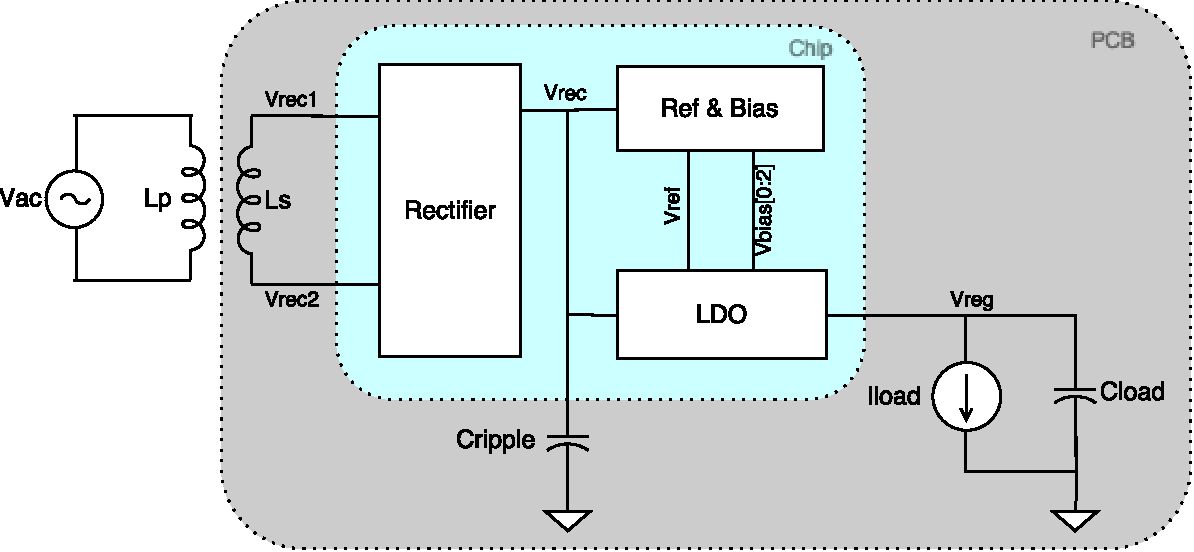
\includegraphics[width=\textwidth]{img/block_diagram.pdf}
   \caption{Block diagram of complete design}
   \label{fig:blockd}
\end{figure}

As shown in the block diagram above, the design includes antennas rectifier, \acrshort{ldo} regulator and reference and biasing circuits. This report mainly discusses about the various design aspect of rectifier and \acrshort{ldo}. The inductor is designed with the specifications provided by NORDIC. The biasing and reference circuit is designed solely for learning the design technique without much effort on the accuracy of the generated biases and references. So externally supplied bias and reference will be the secondary option. The project is designed in tsmc90nm process. Table \ref{proj_spec} lists the main specifications of this project.  \\ 

\begin{table}[!htbp]
\caption{Project specifications}
\begin{center}
\begin{tabular}{c|c}
\hline \hline
Technology 		& TSMC 90nm 9M-1P\\ \hline
Chip area 			& TBA mm\textsuperscript{2} \\ \hline
Input AC voltage	& 2.5 Vp \\ \hline
Operating frequency & 13.56 MHz \\ \hline
Maximum load 		& 10 mA \\ \hline
Output DC voltage 	& 1.8 V \\ 
\hline \hline
\end{tabular}
\end{center}
\label{proj_spec}
\end{table}

A brief discussion of rectifier design is followed next.


\clearpage
\newpage
% *********************************************************************** RECTIFIER  ***********************************************************************

\section{Rectifier}
The most basic rectifier is conventional full wave bridge structure where the diodes are replaced by the diode connected \acrshort{mos}. devices in \acrshort{cmos}. technology. This topology though being simple to implement, has a major drawback. It requires at least twice the $\acrshort{vtn}$ of a MOS device as there are two diode connected MOSes in the conduction path for each cycle of the input signal.  \\

Gate cross coupled and fully gate cross coupled topologies are improvements over conventional full wave rectifier. In gate cross coupled rectifier, two diodes of conventional rectifier is replaced by two gate cross coupled MOSes working as switches where the voltage drop for every cycle is reduced to one threshold voltage. Similarly, in the fully gate cross coupled rectifier, all diodes are replaced by switches and hence the voltage drop is further reduced to twice the conduction drop only for every cycle. Even though this topology has least voltage drop, it suffers from the problem of reverse charge leakage because when the input ac amplitude is less than the output rectified voltage and the conducting pass devices are on simultaneously, current flows backward from output to input. \\

All the above discussed topology suffer from either large voltage drop or large power loss because of which their use are limited in low power and low voltage devices. The popular techniques for higher efficiency are using gate cross coupled rectifier along with passive or active circuitry  for controlling other two pass devices. In passive rectifier, additional circuitry including bootstrap capacitor are used to reduce or eliminate threshold voltage one of which is discussed in this paper \cite{rectboot}. However, use of on-chip bootstrap capacitors limits it use where chip area and speed is of importance. On the other hand, in active rectifier, active circuitry is used control pass devices. The use of active circuitry increase both  \gls{vce} and  \gls{pce} because the pass devices are made to conduct in linear region and hence less conduction drop, and reverse current flow can be completely eliminated and hence less power loss. However active rectifier is not problem free either. The major issue is starting of the active circuit as there is no regulated supply at the start up. \\

\subsection{Design}

In this project, active rectifier is chosen, primarily for better VCE and PCE and secondarily to avoid the use large on chip capacitors. \cite{rectrcc}  and \cite{rectcomp} have discussed same active rectifier topology with a slight difference in active circuitry. \cite{rectrcc} has implemented comparator with compensating the delay of comparator's output falling whereas \cite{rectcomp} has implemented comparator with compensating both the falling and the rising delay of comparator's output in expense of added circuit complexity and power consumption. \cite{rectrcc} has been used here for its simple design. \\

Figure \ref{rect_conv}, \ref{rect_cc} and \ref{rect_rcc} is the CMOS implementation of conventional full wave bridge rectifier, gate cross coupled rectifier and proposed active rectifier in \cite{rectrcc}. The problem with \ref{rect_conv} and \ref{rect_cc} has already been briefly mentioned above. Though  \ref{rect_cc}  is significantly improvement over  \ref{rect_conv} , it is still not a favourable topology with respect to the design technology chosen. In the gate cross couple rectifier of  \ref{rect_cc}, the cross coupled pMOSes act as switches, so the only voltage drop across them is conduction drop due to channel resistance. However the other two nMOSes are diode connected, so they have at least $Vtn$ drop across them which means $Vac \geq Vdc + Vtn$ for conduction. \\

\begin{figure} [htbp]
  \centering 
  \subfloat[Conventional full wave bridge rectifier]  {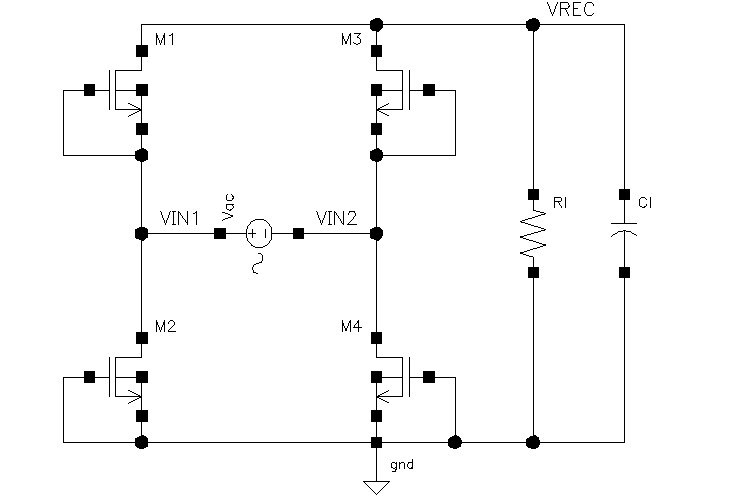
\includegraphics[width=.49\textwidth]{img/rectifier_full_bridge.pdf} \label{rect_conv}}
\hfill
 \subfloat[Gate cross coupled full wave rectifier]  {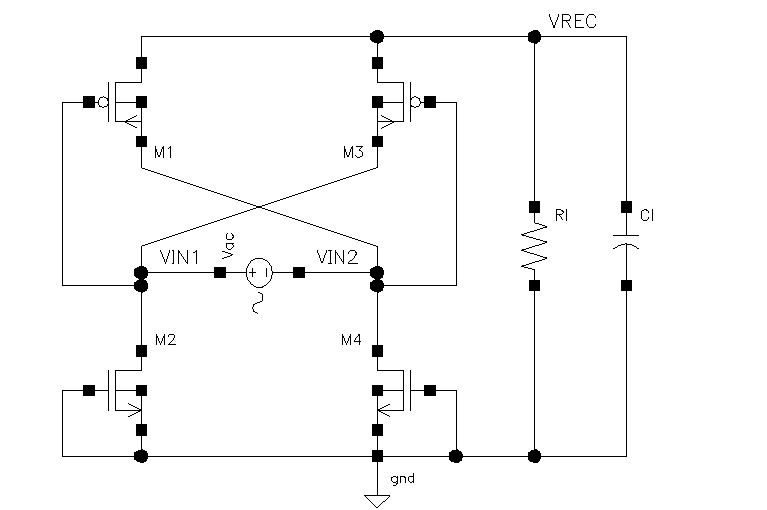
\includegraphics[width=.49\textwidth]{img/rectifier_full_cc.pdf}\label{rect_cc}}
 \caption{Rectifier topologies: conventional and gate cross coupled} 
\label{rect_conv_cc} 
\end{figure}

The proposed active circuit in \ref{rect_rcc} is improvement over \ref{rect_cc} which eliminates $Vtn$ drop required for conduction by replacing diode connected nMOS with devices controlled by active circuit as shown in figure \ref{rcc}. The active circuit is a four input comparator that turns on nMOSes fast when Vac > Vdc and turns off fast to avoid flow of current. \\

For the illustration of operation of comparator, consider the case when $Vin1 > Vin2$ i.e. $Vin1 > 0$ and $Vin2 < 0$. During this half cycle, comparator $D1$ output is low and turns off $Mn2$ and also, $Mp1$ is reversed biased and hence there is no path to flow current along $Mn2$ and $Mp1$. For simplicity, assume $Vac =  Vin1 - Vin2$. When $Vac$ reaches $\acrshort{vtp}$, $Mp3$ turns on which shorts $Vin1$ to $Vrec$. When $Vac > Vrec$, $D2$ output goes high, which turns on $Mn4$ and starts the conduction path for the first half cycle and starts charging $Cl$. When $Vac$ reaches maximum, it starts to decrease and at $Vac < Vrec$, conduction stops as output of $D2$ is low and $Mn4$ is off. As $Vac$ further decreases to below $Vtp$, $Mp3$ if off too. This way rectifier in \ref{rect_rcc}  conducts during positive half cycle eliminating the $Vtn$ drop seen in \ref{rect_cc}. Now the only drop is the conduction drop due to channel resistance of two pass devices along the conduction path. This drop is much less because during conduction both the device are operating in the linear region with small resistance. The operation is similar for $Vin2 > Vin1$ where $Mn4$ and $Mp3$ are off and $Mn2$ and $Mp1$ conduct to charge $Cl$. \\

\begin{figure}[htbp] %figure placement: here, top, bottom, or page
   \centering
   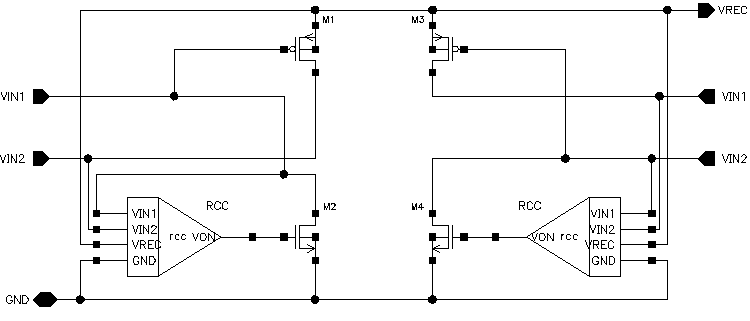
\includegraphics[width=\textwidth]{img/rectifier_schematic.pdf} 
   \caption{Gate cross coupled full wave active rectifer]}
   \label{rect_rcc}
\end{figure}

Figure \ref{rcc}  is the implementation of four input comparator $D2$ used in \ref{rect_rcc} as proposed in \cite{rectrcc}. It is designed to self power and bias because no steady state supply is available at start up. $M1$, $M2$ and $M7$ monitors voltage across $Mn4$ i.e $Vin2 - Vgnd$ and $M3$, $M4$ and $M8$ monitors voltage across $Mp3$ ie $Vin1 - Vrec$ . So when $Vin1 - Vrec > Vin2 - Vgnd$ which means $Vac > Vrec$, output of $D2$ is high and turns on $Mn4$ instantly. But when $Vac < Vrec$, the output of comparator is delayed to fall which causes $Mn4$ to conduct in reverse direction leading to significant reduction in power delivered to load. $M9$ is introduced in order to overcome this problem which adds offset currents to increase $Van$ and $Vpn$ faster, causing the output to decrease faster and turns off $Mn4$ before $Vac < Vrec$. This reverse current control technique compensates the comparator delay and increases the power efficiency of the rectifier. \\

\begin{figure}[htbp] %figure placement: here, top, bottom, or page
   \centering
   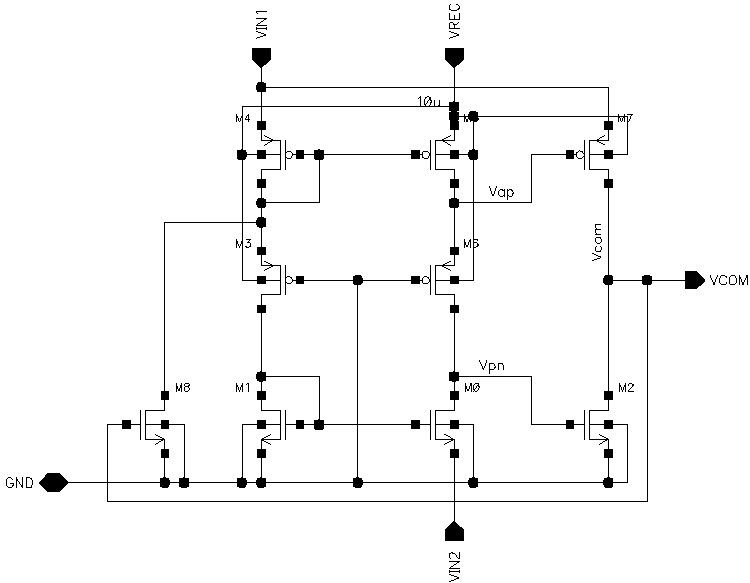
\includegraphics[width=\textwidth]{img/rectifier_rcc5.pdf} 
   \caption{Comparator circuit, RCC }
   \label{rcc}
\end{figure}

The design parameters for the rectifier is listed in table  \ref{tab:rect_parameter}. The dimensions of the pass devices are first hand calculated by using square law current equation and devices parameters values given in the technology documents, and later optimised with simulation tool in order to make the rectifier to deliver the required current. Since \acrshort{nmos} does not have to have same device size as \acrshort{pmos} to deliver same current, optimal size ratio equation from \cite{rectsize} is used to find nMOS pass devices sizes. Thought maximum load for this work is 10 mA, It is always simulated with 1 mA extra load. This extra current is to account for the fact that RCC is self powered and LDO which will follow this rectifier will be powered by $Vrec$. Similarly, the value of ripple rejection capacitor is chosen 100nF. This size of 
filter capacitor is calculated from capacitor current-voltage relationship with the assumption of keeping peak to peak ripple voltage below 5 mV to deliver 11 mA current.  \\

\begin{table}[H]
\caption{Rectifier design parameters}
\begin{center}
\begin{tabular}{c|c}
\hline \hline
Wn/Ln, Wp/Lp 		& 720um/280nm, 1.2mm/280nm \\ \hline
Rectifier area 		& TBA mm\textsuperscript{2} \\ \hline
Operating frequency 	& 13.56 MHz \\ \hline
Input ac magnitude	& 2.5  \acrshort{vp}\\ \hline
Load current 		& 11 mA \\ \hline
Ripple rejection capacitor	& 100 nF \\ 
\hline \hline
\end{tabular}
\end{center}
\label{tab:rect_parameter}
\end{table}

\subsection{Transient performance}

Figure \ref{rect_tb} is the test bench setup for simulation of the rectifier. Figure \ref{rect_plot} show the simulation results showing voltages at the input ac and output rectified DC 
voltages and current through rectifying MOSes. These  
waveforms clearly follows the working principle discussed above. Two important observations can be made from 
plots. First, the rectified output $Vrec$ is 2.2 V for $Vpp$ ac input of 2.5 V for driving which means the 
voltage loss has been significantly reduced and the loss of around 300 mV yields to the conduction loss due 
the channel resistance. Secondly, the reverse current from output to input has been effectively eliminated as 
there is only positive current flowing to the load when all conducting devices 
are on.  \\

\begin{figure}[htbp] %figure placement: here, top, bottom, or page
   \centering
   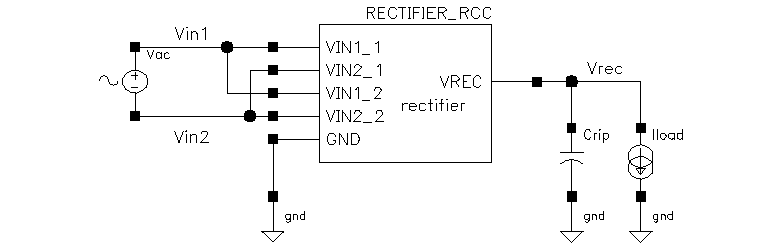
\includegraphics[width=\textwidth]{img/rectifier_testbench.pdf} 
   \caption{Testbench for rectifier}
   \label{rect_tb}
\end{figure}

\begin{figure}[H] %figure placement: here, top, bottom, or page
   \centering
   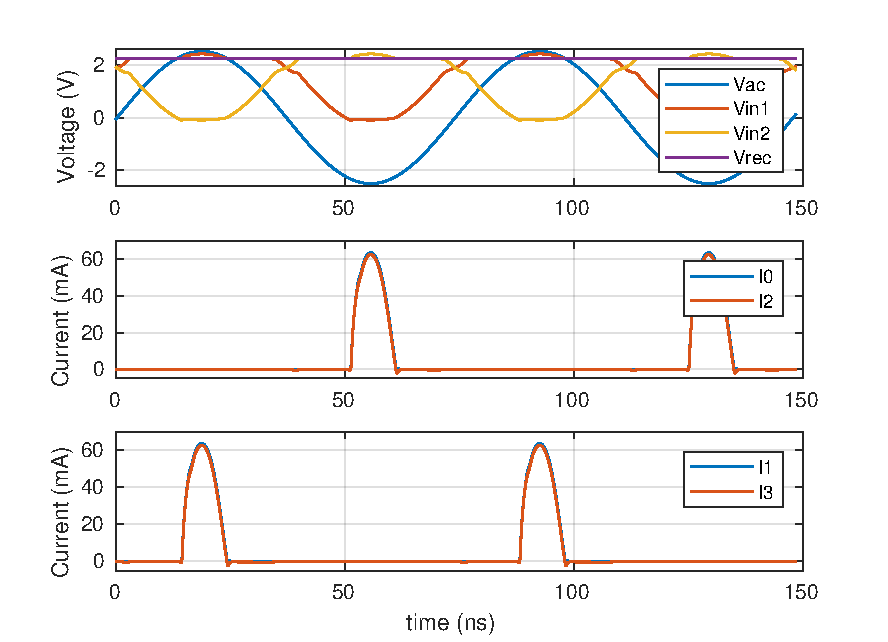
\includegraphics[width=\textwidth]{img/rectifier_VI.pdf} 
   \caption{Voltage and current waveforms of the rectifier}
   \label{rect_plot}
\end{figure}

Figure  \ref{fig:rect_v_post}  presents both pre and post layout results of input voltages, $Vin1$ and $Vin2$  and output voltage, $Vrec$, for one cycle of ac input. The closer view of rectified output is shown in figure \ref{fig:rect_ripple}. The voltage drop of about 60 mV in layout result is accounted for the voltage drop due to 
the resistance of high current conduction path. \\

\begin{figure}[H] %figure placement: here, top, bottom, or page
   \centering
   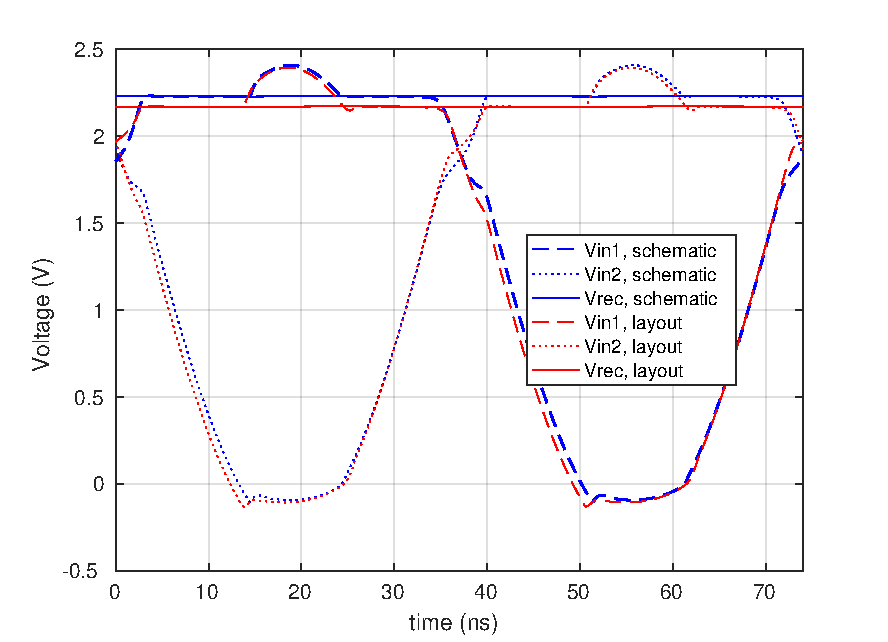
\includegraphics[width=\textwidth]{img/rectifier_V_post.pdf} 
   \caption{Voltages waveform for pre and post layout}
   \label{fig:rect_v_post}
\end{figure}

\begin{figure}[H] %figure placement: here, top, bottom, or page
   \centering
   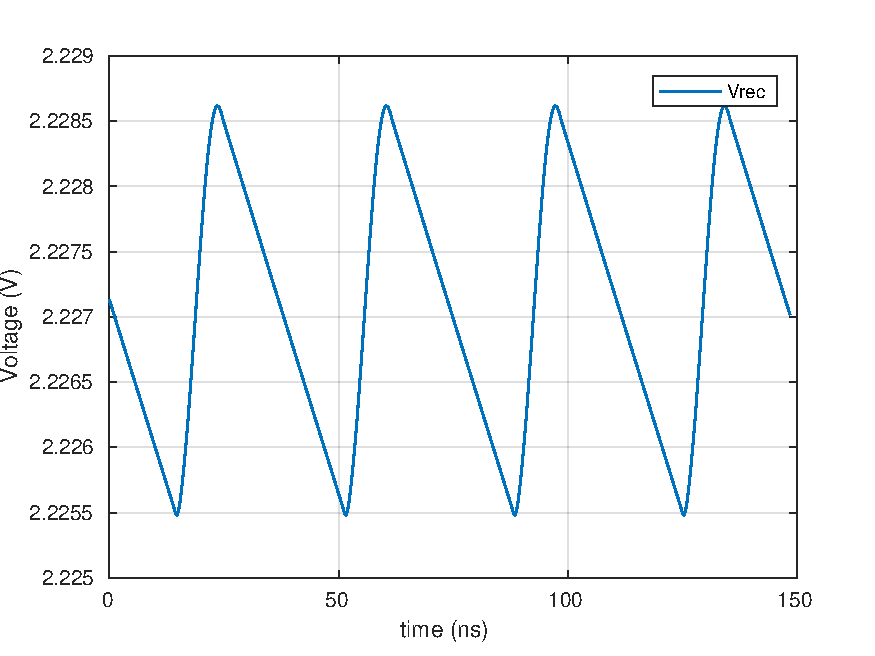
\includegraphics[width=\textwidth]{img/rectifier_ripple.pdf} 
   \caption{Rectified DC output for pre and post layout}
   \label{fig:rect_ripple}
\end{figure}

\subsection{DC performance}

Similarly, figure  \ref{rect_ce} shows PCE, ratio of powered delivered to load to average power from the source and 
VCE, ratio of rectified DC, $Vrec$ to peak ac input, |$Vac$| with respect to magnitude peak ac input signal. |$Vac$| is gradually increased in 
peak magnitude in step of 50 mV and VCE and PCE is calculated for every step. The plot shows both 
PCE and VCE are very less for input ac amplitude less then 1.8 V. It can be explained by the fact that required 
bias current and gate drive voltage for RCC circuit are not achieved for smaller input. [INCLUDE POST LAYOUT RESULT TOO] \\

\begin{figure}[htbp] %figure placement: here, top, bottom, or page
   \centering
   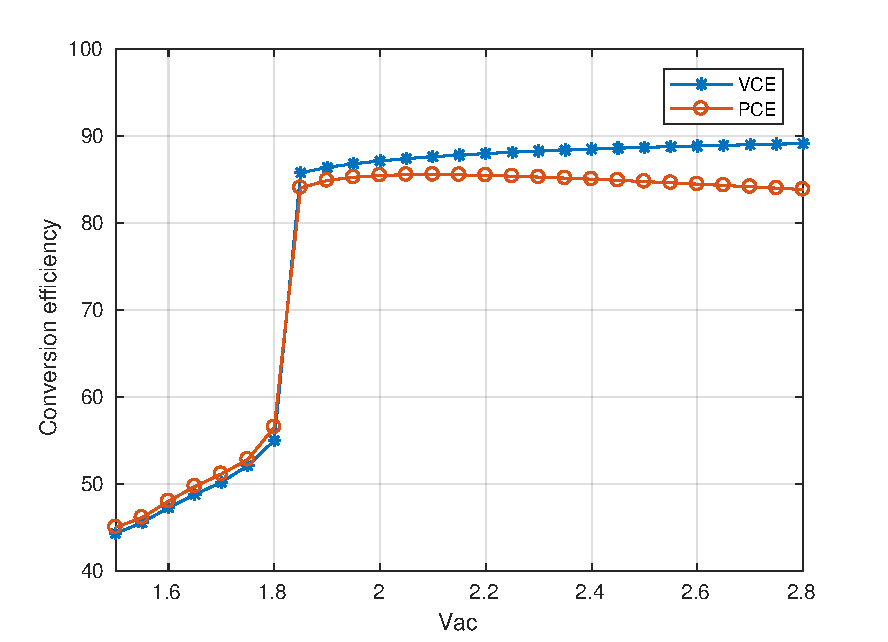
\includegraphics[width=\textwidth]{img/rectifier_ce.pdf} 
   \caption{Voltage and power conversion efficiency}
   \label{rect_ce}
\end{figure}

Table \ref{tab:rect_spec} comparatively summarises performance for pre and post layout result of the design. The layout design is attached in appendix. The layout 
is made symmetrical with four inputs, as seen in test bench figure \ref{rect_tb}, instead of two. This is done to make the current conducting path equal which result in 
equal drop in voltage when it reaches the rectifying MOSes. Simialarly the paths from the pad to the recitifier inputs are mask blocked for random metal fill to avoid 
inter layer coupling [WHY???]. The high current conduction routes are designed with wide parallel path of many higher level metal layers for reducing resistance in conduction path.

\begin{table}[H]
\caption{Rectifier performance summary}
\begin{center}
\begin{tabular}{c|c|c}
\hline \hline
				 & \textbf{Schematic}		& \textbf{Post-layout} \\
\hline \hline
Rectified DC	 	& 2.23 V 				& 2.17 V	\\ \hline
Ripple \acrshort{vpp} & 3.1 mV 				& 3 mV	\\ \hline
Peak diode current 	& 63.7 mA 			&	-	\\ \hline
PCE 				& 84.5 \% 				&	-	\\ \hline
VCE 				& 88.6 \% 				&	86.2 \%	\\
\hline \hline
\end{tabular}
\end{center}
\label{tab:rect_spec}
\end{table}


\clearpage
\newpage
% *********************************************************************** LDO  ***********************************************************************

\section{LDO}

Voltage regulator follows the rectifier designed above in order to regulated the rectified voltage to 1.8 V and 
deliver maximum load current of 10 mA. Since the output from the active rectifier is 2.2 V and the required 
regulated voltage is 1.8 V, charge pump or  \acrshort{smps} of boost type is irrelevant here. Buck SMPS could be 
an option for voltage regulation but LDO is preferred for it better performance in terms of noise and faster 
settling of regulated voltage.  \cite{ldo_psu}.\\ 

Figure \ref{ldo_gen} shows a circuit of typical LDO with pMOS as pass element. As shown in the figure, the 
components includes an error amplifier (EA), a pass device (Mpass), a feedback circuit (R1 and R2) and load 
(C\textsubscript{out} and I\textsubscript{load}). A more general and complete LDO circuit also includes 
circuitry for generation of reference voltage and bias current/voltage. In this project it will be discussed 
separately later. The working principle of LDO is that the error amplifier compares the scaled down regulated 
voltage, Vdiv with Vref and regulates the internal resistance of the pass transistor such that  the error, 
V\textsubscript{ref} - V\textsubscript{div} is least or zero ideally. \\

\begin{figure}[htbp] %figure placement: here, top, bottom, or page
   \centering
   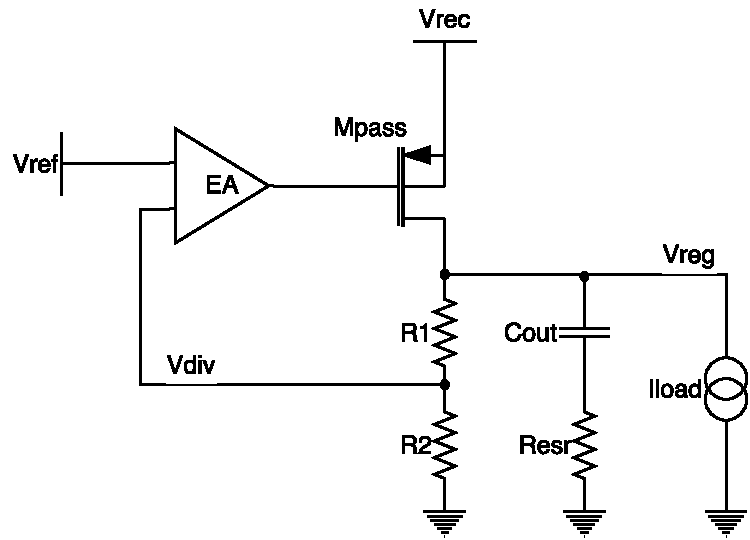
\includegraphics[width=.9\textwidth]{img/ldo.pdf} 
   \caption{Generic LDO with pMOS pass device}
   \label{ldo_gen}
\end{figure}

\cite{ldo_bulkmod} and \cite{ldo_quiescent} are two examples of CMOS implementation of LDO. \cite{ldo_bulkmod} 
has proposed bulk modulation technique for improving load regulation and stability of capacitor-less LDO. 
Similarly \cite{ldo_quiescent} has  proposed techniques for increasing current efficiency of LDO especially at 
no or low load condition. Though the techniques discussed in these designs have not been used, they have given 
good insight into different design parameters of LDO.  \\

\subsection{Design}

Figure \ref{ldo_cmos} shows the CMOS implementation of LDO in this project. The components in this design 
include a folded cascode differential amplifier as error amplifier, pMOS buffer, pMOS pass device and feedback 
network of resistors. \\

\begin{figure}[htbp] %figure placement: here, top, bottom, or page
   \centering
   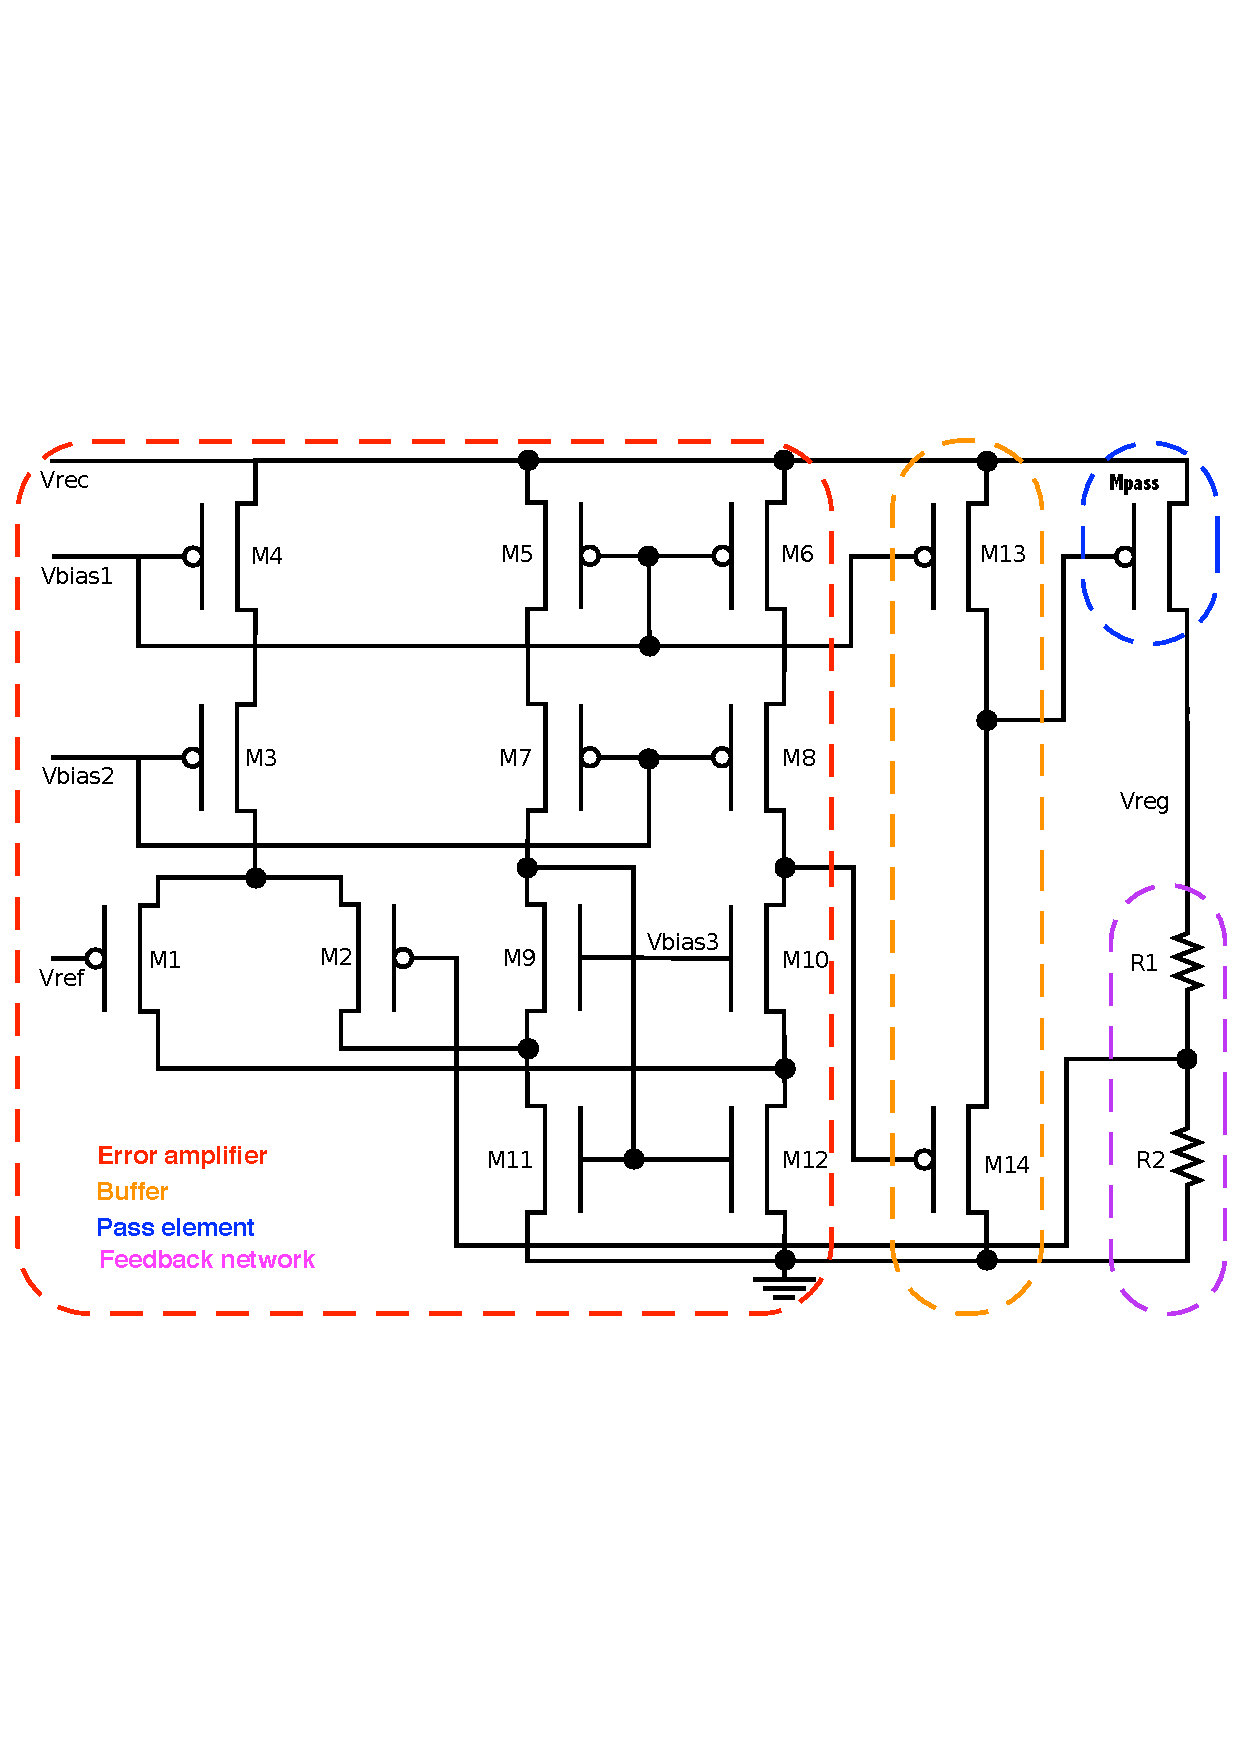
\includegraphics[width=0.9\textwidth]{img/sch_ldo_label.pdf} 
  %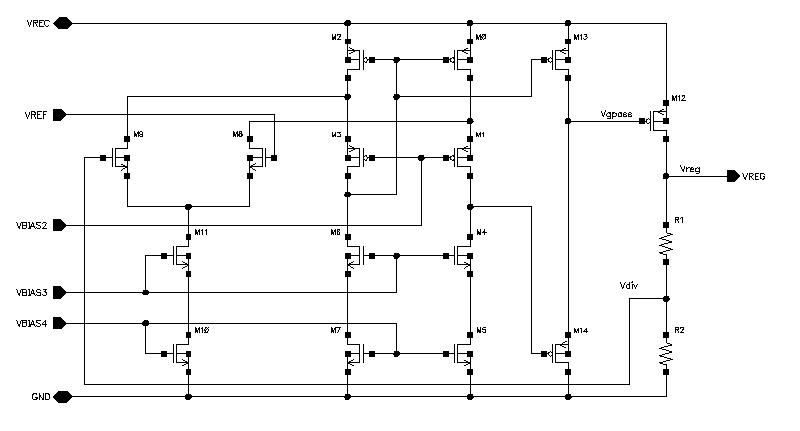
\includegraphics[width=0.9\textwidth]{img/ldo_schematic.pdf} 
   \caption{CMOS implemenation of LDO}
   \label{ldo_cmos}
\end{figure}

As briefly mentioned above, the error amplifier amplifies the error i.e. difference in scaled regulated voltage, 
V\textsubscript{div} and reference voltage, V\textsubscript{ref}. It is known that an amplifier with higher 
open loop \acrshort{dc} gain reduces the closed loop gain error and hence amplifier with higher gain is desired 
here which is turn increase the accuracy of regulated voltage, Vreg \cite{ldo_bulkmod}. Typically error amplifier 
has gain $> 40 dB$ which is not achieved with a single stage amplifier with this technology. Higher gain can be 
achieved by cascading multiple single stage but with increased difficulty in making the multistage
amplifier stable. So for achieving higher DC gain and at the same time for stability convenience, folded cascode 
amplifier \cite[pp. xx]{razavi_2001} is chosen. \\

\begin{table}[H]
\caption{LDO design parameters}
\begin{center}
\begin{tabular}{c|c}
\hline \hline
Pass device				& pMOS \\ \hline
(Wp/Lp)\textsubscript{pass} 	& 540um/280nm \\ \hline
Input supply 				& >2.2 V \\ \hline
Error amplifier				& folded cascode \\ \hline
Vbias2 					& 1.1 V \\ \hline
Vbias3					& 0.88 V \\ \hline
Vbias4					& 0.68 V \\ \hline
Vref						& 1.17 V \\ \hline
C\textsubscript{load} 		& > 2.5 \si{\micro\farad}  \\ \hline
R\textsubscript{esr} 	 		& > 0.8 $\Omega$ \\ \hline
Regulated output voltage 		& 1.8 V \\ \hline
I\textsubscript{load} max. 		& 10 mA \\
\hline \hline
\end{tabular}
\end{center}
\label{tab:ldo_parameter}
\end{table}


The amplifier has a nMOS differential input stage, perferably for its higher mobility for achieving more gain.
Reference voltage, V\textsubscript{ref} will be bandgap voltage, 1.17 V, of silicon and  thus \acrshort{icmr} 
for EA lies almost at half the supply voltage. This amplifier drives a pMOS buffer which is used to supply 
sufficient current to drive the large pass transistor. Moreover, pMOS as a buffer passes 1 better which means 
it can turn off the pass device completely and hence LDO regulates better at low load or no load condition. 
However for heavier load/larger load current, this pMOS buffer is not able to pull down the gate of pass device 
suffuiciently lower. This is overcome by making the pass device large enough to feed the required  maximum 
load current.\\

The pass device is a pMOS transistor in this design. It is chosen because it has several advantages over it's 
counterparts like nMOS and BJT devices in terms of dropout voltage, quiescent current, input voltage, thermal 
response and noise\cite{ldo_ti_pmos}. Prominently, there are two factors that give pMOS edge over other devices; 
dropout voltage and quiescent current, when it comes to application in low power and low voltage devices. nMOS as 
a pass device requires a positive drive voltage with respect to output to operate. On the other hand, pMOS is 
driven by a negative signal with respect to input which means pMOS is preferable for a low input LDO. Similarly 
compared to BJTs, pMOS requires less headroom and less quiescent current to be driven\cite{ldo_ti_pmos}, 
\cite{ldo_ti_stability}, which means low dropout and low power operation, typical requirement of today's micro 
devices' power supply. \\

\begin{figure}[htbp] %figure placement: here, top, bottom, or page
   \centering
   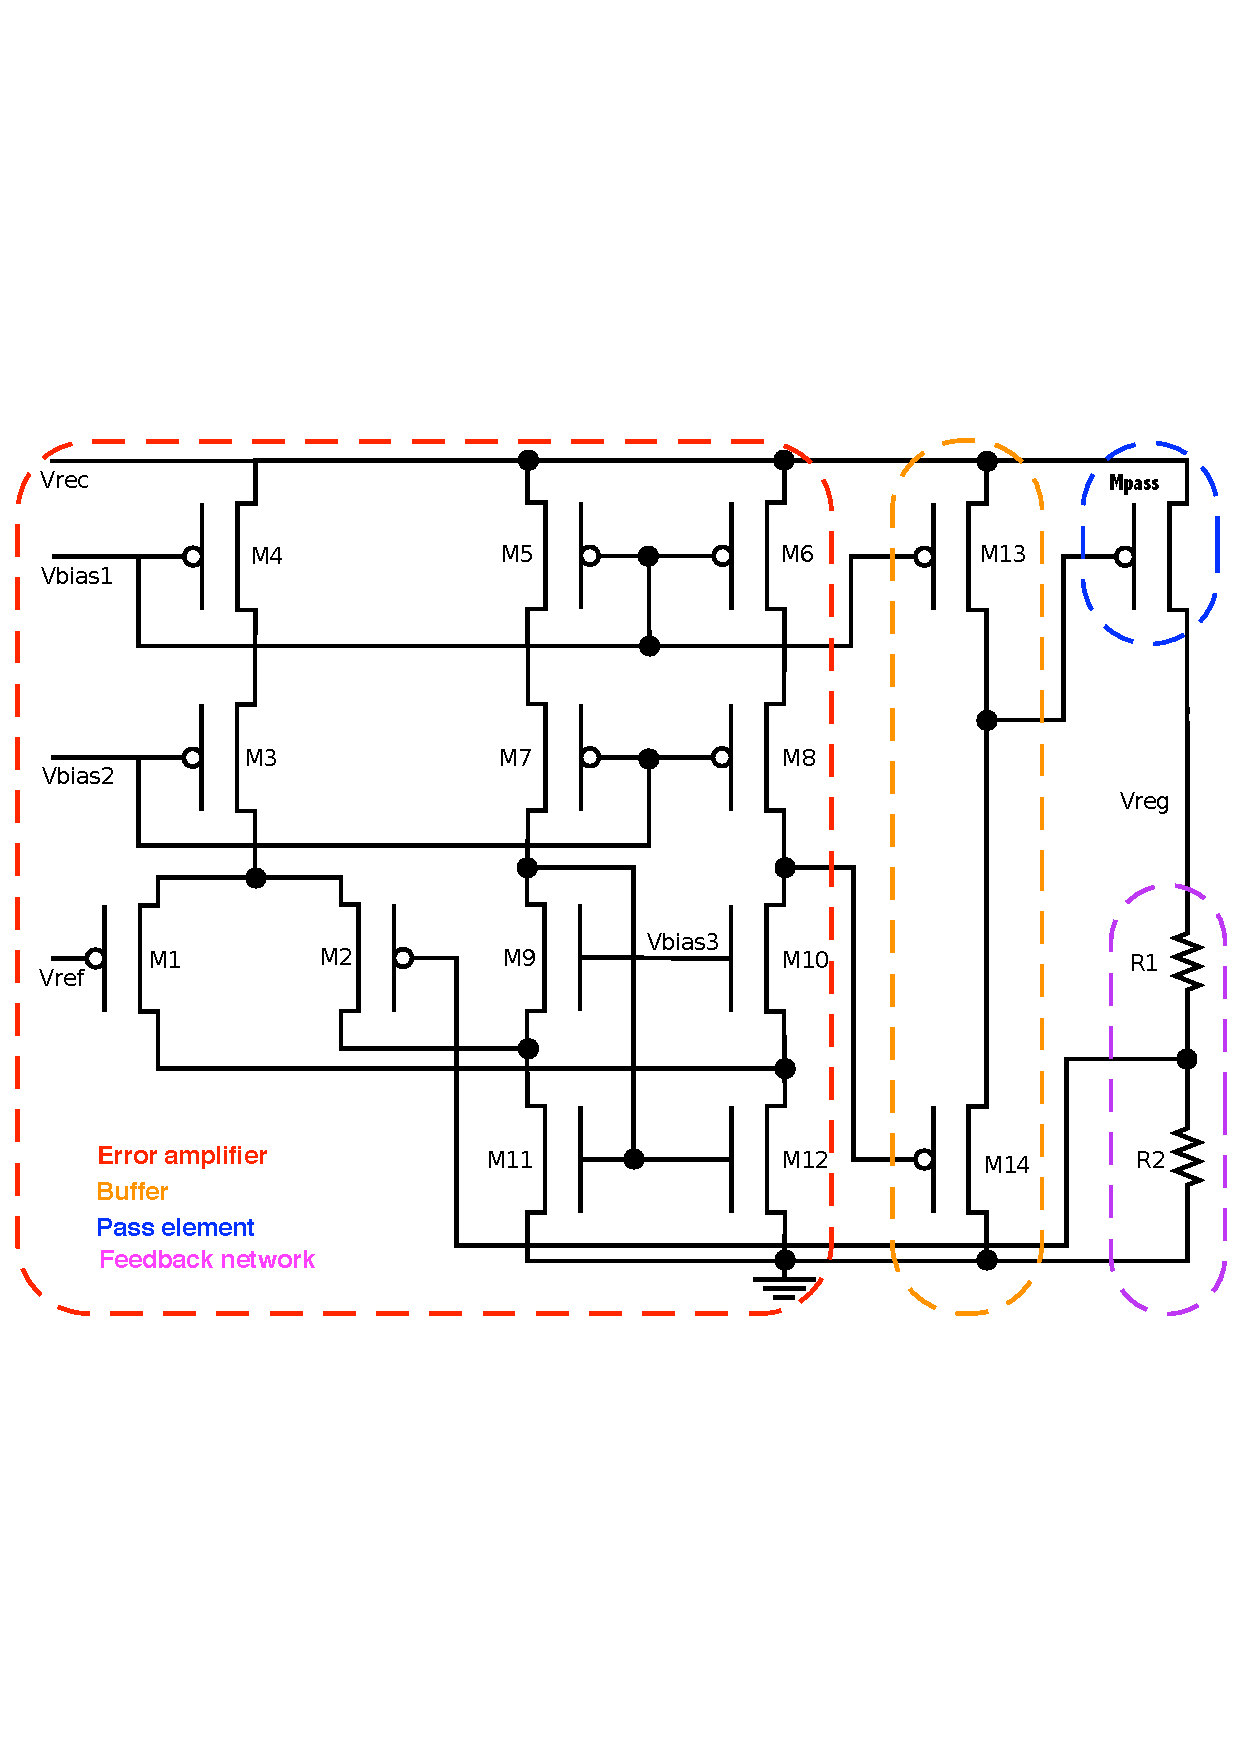
\includegraphics[width=0.9\textwidth]{img/sch_ldo_label.pdf} 
   \caption{LDO testbench setup}
   \label{fig:ldo_testbench}
\end{figure}

However, pMOS as a pass device in LDO causes challenges in stability. As mentioned above, LDO utilises a high 
gain feedback loop in order to provide a regulated output voltages independent of load current and in any system 
with feedback loop, the locations of poles and zeros determine stability of the system.  In case of the pMOS LDO, 
the pass device is configured in a common source configuration. LDO with big output cap has a dominant pole pole 
at the output, which is a low frequency pole. The second pole is located at the gate of pass device because as 
mentioned earlier pMOS pass device is large and has a big parasitic capacitance. This second pole may be located 
closer to the dominant pole, resulting in significant  reduction in phase margin (\acrshort{pm}). Consequently, 
this may lead to instability of the LDO with pMOS pass device.  Various methods have been implemented for 
ensuring the stability of the pMOS LDO. In this project, a large external capacitor, $C\textsubscript{load}$ in 
figure \ref{ldo_gen}, is used for stabilising the system at the cost of additional settling time. When an 
external capacitor is used for designing a stable LDO, the minimum value of capacitance, $C\textsubscript{load}$ 
and minumum value of its equivalent series resistance (\acrshort{esr}), $R\textsubscript{esr}$ should be 
specified\cite{ldo_ti_stability}. $C\textsubscript{load}$ determines the dominant pole of the LDO and 
$R\textsubscript{esr}$ in series with $C\textsubscript{load}$ introduces a left half plane zero below unity 
gain frequency, \acrshort{ugf} of LDO in order to cancel out the non-dominant pole below UGF, producing a 
stable LDO system. \\

\subsection{Transient response}

Figure \ref{fig:ldo_tran} is the transient simulations of the LDO which illustrates generation of  regulated output voltage, $Vreg$ for 
both maximun load, 10 mA. For maximum load, it takes minimum 107 us to produce stable voltage. Since a large capacitor is used for stabilising 
LDO, it take longer time. Compared to schematic result, it takes 9 us extra time which can be accounted additional parasitic capacitance of interconnects 
at the output of LDO.\\

\begin{figure}[H] %figure placement: here, top, bottom, or page
   \centering
   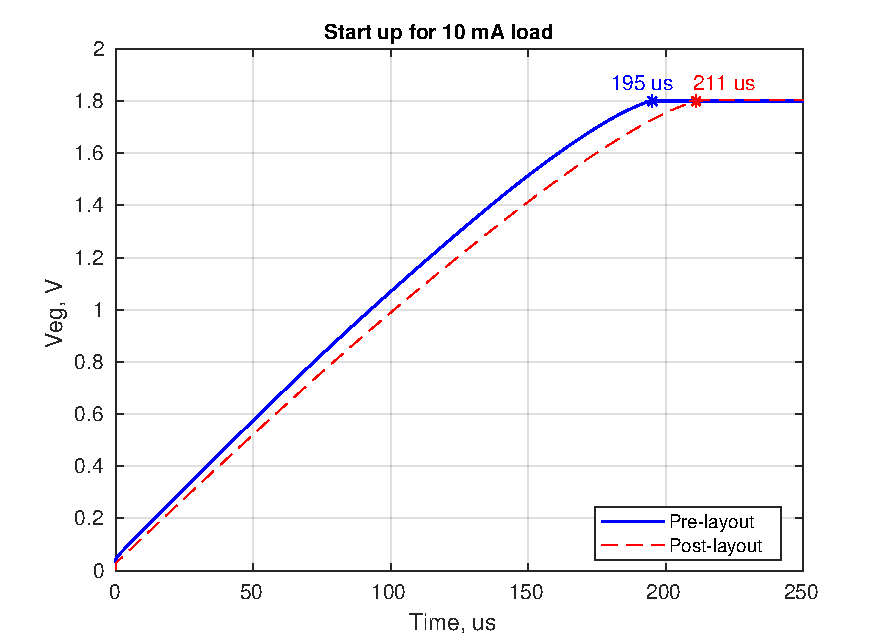
\includegraphics[width=\textwidth]{img/ldo_transient_both.pdf} 
   \caption{LDO transient simulation}
   \label{fig:ldo_tran}
\end{figure}

Figure \ref{fig:ldo_loadr} and \ref{fig:ldo_liner} show the transient response of LDO for line, $Vrec$ and load, $Iload$ variation. 
It gives information about how well and how fast regulated output settles for line and load variations. In  figure \ref{fig:ldo_loadr} load is given as pulse
 varying from 10 uA to 10 mA with both falling and rising time of 1 ns keeping input supply constant to 2.2 V. Sudden increase in load causes the output voltage to drop. The error amplifier then takes some time adjusts the gate voltage of pass device to low to fully turn on the device. Likewise when the load suddenly drops to minimum, it causes the output voltage to increase. Again error amplifier adjust it back by increasing the gate voltage of pass device to turn it off. Similarly for line variation 
 observation, input, $Vrec$ is pulsed from 2 V to 2.5 V with 1 ns rising and falling time keeping load current constant to 10 mA. Sudden increase in input voltage causes output to increase and vice-versa. As in load variation case, similar recovery pattern is seen. In both case of load and line regulation, the out put voltage is maintained 
 quickly, less than 0.15 us. Both results from schematic and post layout have same transition behaviour except post layout result offset by 3.7 mV as explained in DC response section below. \\
 
  Line regulation, change in regulated output voltage due to maximum change in input voltage and load regulation, change in output voltage due to maximum change in 
  load current are calculated from values shown in respective plots and are listed in table \ref{ldo_spec}.

\begin{figure}[H] %figure placement: here, top, bottom, or page
   \centering
   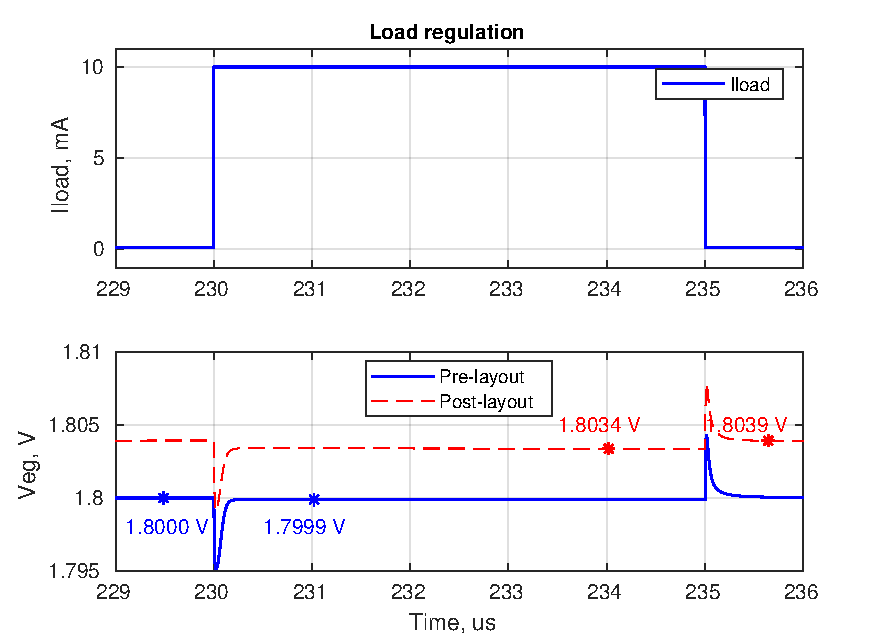
\includegraphics[width=\textwidth]{img/ldo_loadr_both.pdf} 
   \caption{LDO step load regulation}
   \label{fig:ldo_loadr}
\end{figure}

\begin{figure}[H] %figure placement: here, top, bottom, or page
   \centering
   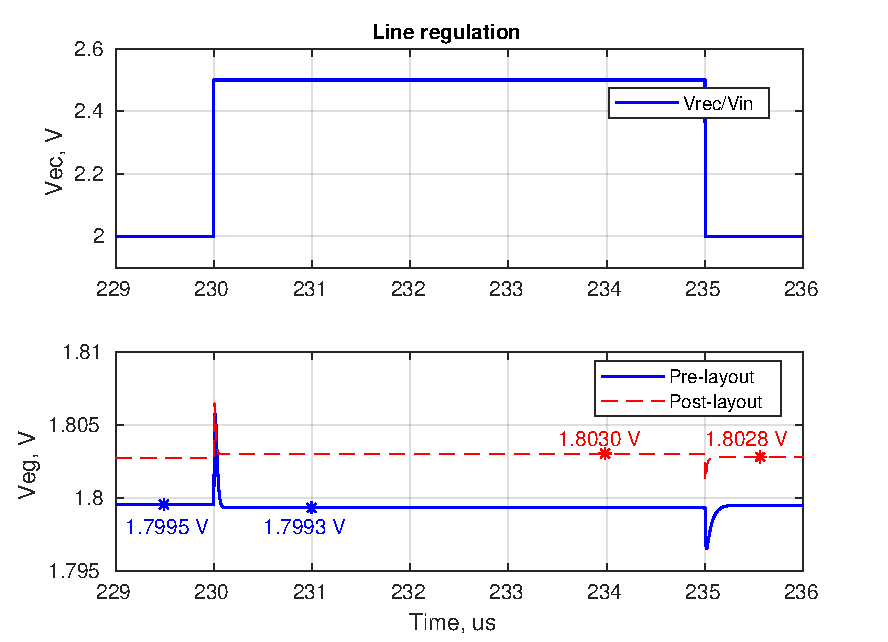
\includegraphics[width=\textwidth]{img/ldo_liner_both.pdf} 
   \caption{LDO step line regulation}
   \label{fig:ldo_liner}
\end{figure}

\subsection{DC response}

Figure \ref{fig:ldo_dc} and \ref{fig:ldo_Iload} show LDO response to input voltage, $Vrec$ sweep and output load, $Iload$ sweep. As seen in \ref{fig:ldo_dc}, the
regulator is turned off for input below 1.85 V. Since the input is also the supply for the entire design, higher voltage is required for creating proper biasing 
of internal folded cascode error amplifier. However after turning on, it requires only 100 mV drop for proper regulation for maximum load and is even lesser for lighter 
load. This shows that minimum value of supply required for LDO to function properly is 1.95 V. In \ref{fig:ldo_Iload}, it is seen that regulated output voltage for post 
layout simulation is 3.7 mV higher than for schematic. Since $Vreg = (1 + R1/R2)*Vref$, the mismatch in the resistors has resulted in slightly higher ratio, consequently 
increasing the close loop gain.\\



\begin{figure}[H] %figure placement: here, top, bottom, or page
   \centering
   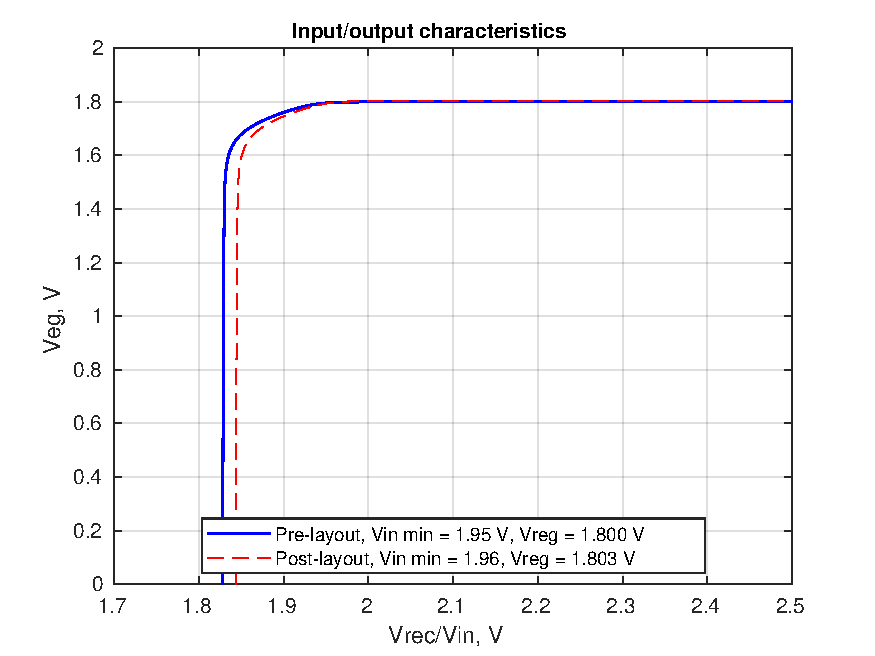
\includegraphics[width=\textwidth]{img/ldo_dc_both.pdf} 
   \caption{Regulated voltage with supply variation}
   \label{fig:ldo_dc}
\end{figure}

\begin{figure}[H] %figure placement: here, top, bottom, or page
   \centering
   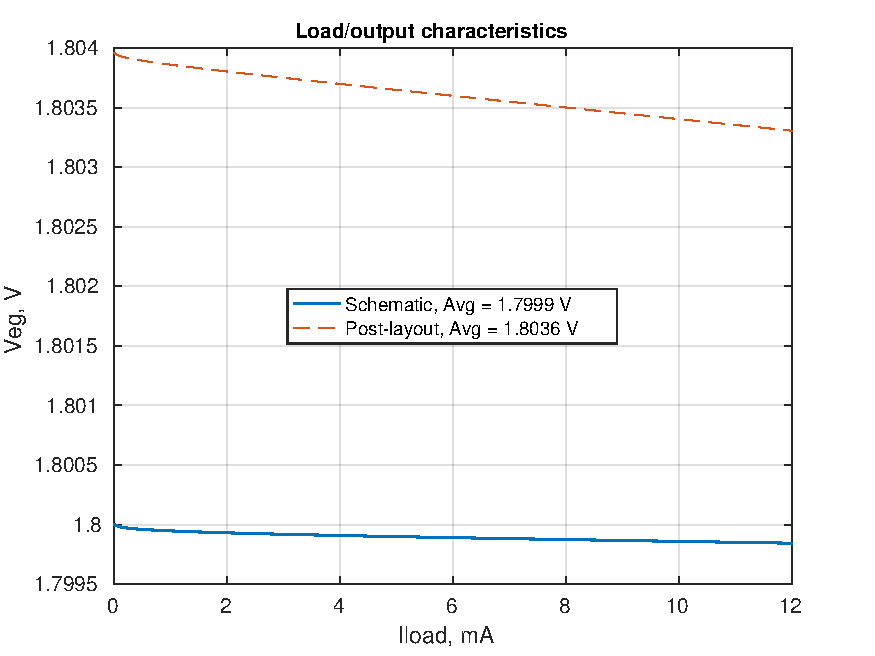
\includegraphics[width=\textwidth]{img/ldo_Iload_both.pdf} 
   \caption{Regulated voltage with load variation}
   \label{fig:ldo_Iload}
\end{figure}

\subsection{AC response}

Figure  \ref{fig:ldo_sta} is open loop gain and phase margin of LDO without and with compensation. In the upper  uncompensated bode plot, two poles below UGF are seen: 
the first one at 300 KHz due to output resistance of pass device and its parasitic capacitance, and the second one at  60 MHz due to buffer output resistance and gate 
capacitance of pass device. UGF is at 100 MHz. Due to these two poles both occurring below UGF, the PM fallen to -45\textdegree. For making the LDO stable, as discussed  in the beginning, a capacitor, $C\textsubscript{load}$, 2.5 uF with specific series equivalent resistance, $R\textsubscript{esr}$, 0.8  $\Omega$ is used at the output.  $C\textsubscript{load}$ and pass device output resistance creates the dominant pole at 1 KHz and $R\textsubscript{esr}$ and $C\textsubscript{load}$ creates a left half plane zero below UGF which cancels the non dominant pole.  This eventually gives 75\textdegree PM and 30 dB \acrshort{gm}. \\ 

Likewise figure \ref{fig:ldo_pssr} is the plot showing \acrshort{pssr}  of this LDO. It can be seen that it has poor PSSR performance for frequency higher than 200 KHz. Low frequency noise like 50Hz supply ripple is effectively rejected. In this design 13.56 MHz ripple and its first harmonics is expected in the input of LDO because rectified 
output from rectifier operating at 13.56 MHz as input signal is used as supply and/or input for this LDO. Unfortunately, PSSR performance is worst around this 
frequencies. However the ripple rejection is still -36 dB at 13.56 MHz which is decent. As seen in figure \ref{fig:ldo_sta}, the open loop gain of LDO feedback circuit is 
90 dB, which has contributed in achieving decent PSSR even at higher frequency\cite{ldo_ti_pssr}. This paper also discusses that UGF frequency corresponds to the roll 
off frequency of PSSR, which can also been seen by comparing plots  \ref{fig:ldo_sta} and \ref{fig:ldo_pssr}. The stability technique in this design also gives adverse effect on PSSR performance as UGF is significantly lowered by large output capacitor. 
\\ 
 
\begin{figure}[H] %figure placement: here, top, bottom, or page
   \centering
   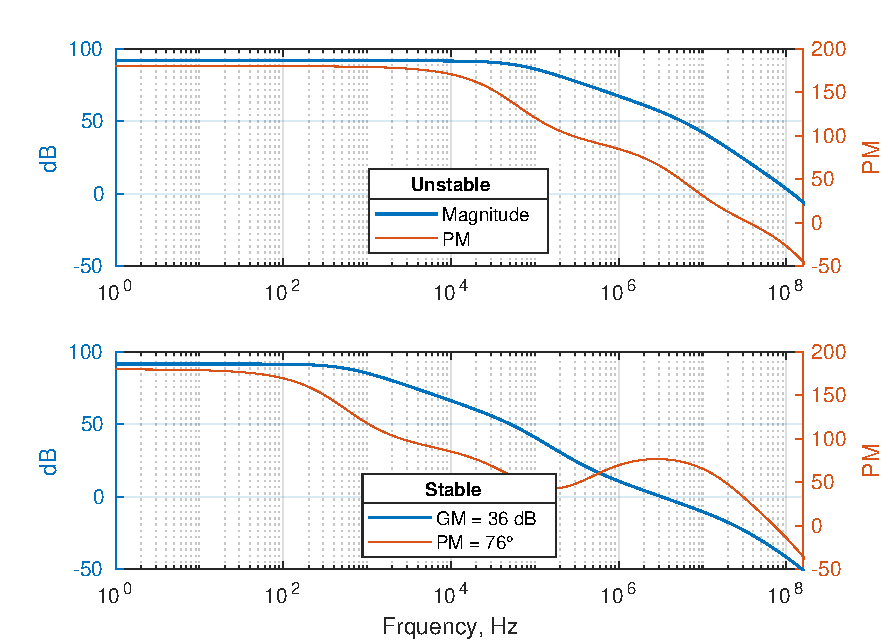
\includegraphics[width=\textwidth]{img/ldo_ac.pdf} 
   \caption{LDO stability before and after compensation}
   \label{fig:ldo_sta}
\end{figure}

\begin{figure}[H] %figure placement: here, top, bottom, or page
   \centering
   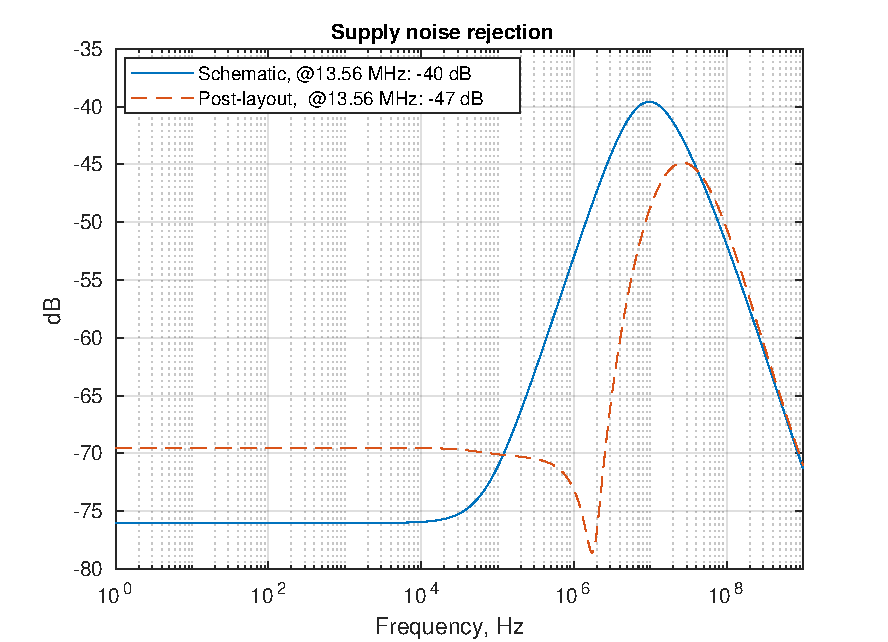
\includegraphics[width=\textwidth]{img/ldo_pssr_both.pdf} 
   \caption{PSSR performance}
   \label{fig:ldo_pssr}
\end{figure}

Table \ref{ldo_spec} summaries the performance of LDO regulator discussed above. Power efficiency is calculated as power delivered to load to power consumed 
from the source. Quiescent current includes biasing currents for error amplifier, feedback resistors and buffer which is obtained by taking the difference of current 
drawn from the source and current delivered to the load. Both power efficiency and quiescent current is calculated for maximum load operation. 

\begin{table}[H]
\caption{LDO performance summary} 
\begin{center}
\begin{tabular}{c|c|c}
\hline \hline
				 & \textbf{Schematic}		& \textbf{Post-layout} \\
\hline \hline
PSSR 			 & -36 dB	@ 13.56 MHz	&-59 dB	@ 13.56 MH\\ \hline
Phase margin		 & 75\textdegree 		&	 \\ \hline
Gain margin		 & 30 dB				&	 \\ \hline
Power efficiency		& 80.9 \%			& 81 \%	\\ \hline
Quiescent current	& 105 uA			& 114 uA	\\ \hline
Load regulation 	& 17 uV/mA			& 53 uV/mA	\\ \hline
Line regulation 		&  435 uV/V 		& -1.162 mV/V	\\ 
\hline \hline
\end{tabular}
\end{center}
\label{ldo_spec}
\end{table}%

Reference and biasing circuit design follows next. \\


\clearpage
\newpage
% *********************************************************************** REFERENCE AND BIASING  ***********************************************************************

\section{Reference and biasing}

Reference and biasing circuit is important part of any analog circuit. It is required to bias the designed circuitry with proper voltages and currents for operating all the devices in the intended region. For reliable and consistent  performance of the system, the references and biases should be independent of supply voltage and temperature variations. Moreover with the trend of shrinking device sizes, mismatch and process parameters variations have been so pronounced that these factors affect the operation of the devices. So for the todays' devices, it is necessary to design reference and biasing independent of \acrshort{pvt} variations. \\

There are different methods of generating reference voltages and bias currents discussed in literatures. Basically, supply independent current source is generated first and then this current is passed through a resistor to get a reference voltages. Some ways of creating supply insensitive current sources are threshold voltage referenced, diode ($V_{BE}$ in BJT) referenced thermal voltage referenced current sources \cite[pp. 305-315]{gray_2009}. However, these current sources are not temperature independent. Threshold voltage of MOS and forward voltage of diode or $V_{BE}$ have a negative temperature coefficient \acrshort{tc}  and hence they produce a \acrshort{ctat} (complementary to absolute temperature) current. On the other hand, the thermal voltage($V_T$) has positive TC and hence it produce a \acrshort{ptat} (proportional to absolute temperature) current. So these techniques, though being insensitive to supply variations, still cannot be used for accurate reference voltage generation because of temperature dependence. So \gls{bgr} design is used to generate the required reference voltage for the LDO in this design which has significantly less PVT variations than the last three methods.\\

BGR design involves summing up two voltages of which one is PTAT and the other is CTAT, both having equal and opposite TCs. The equal and opposite TCs cancels out leaving the resultant voltage with a zero TC. Figure  \ref{bgr_sch} is the CMOS implementation of reference and biasing circuit for this project which includes startup circuit, BGR circuit and biasing circuit. \\

\begin{figure}[htbp] %figure placement: here, top, bottom, or page
   \centering
   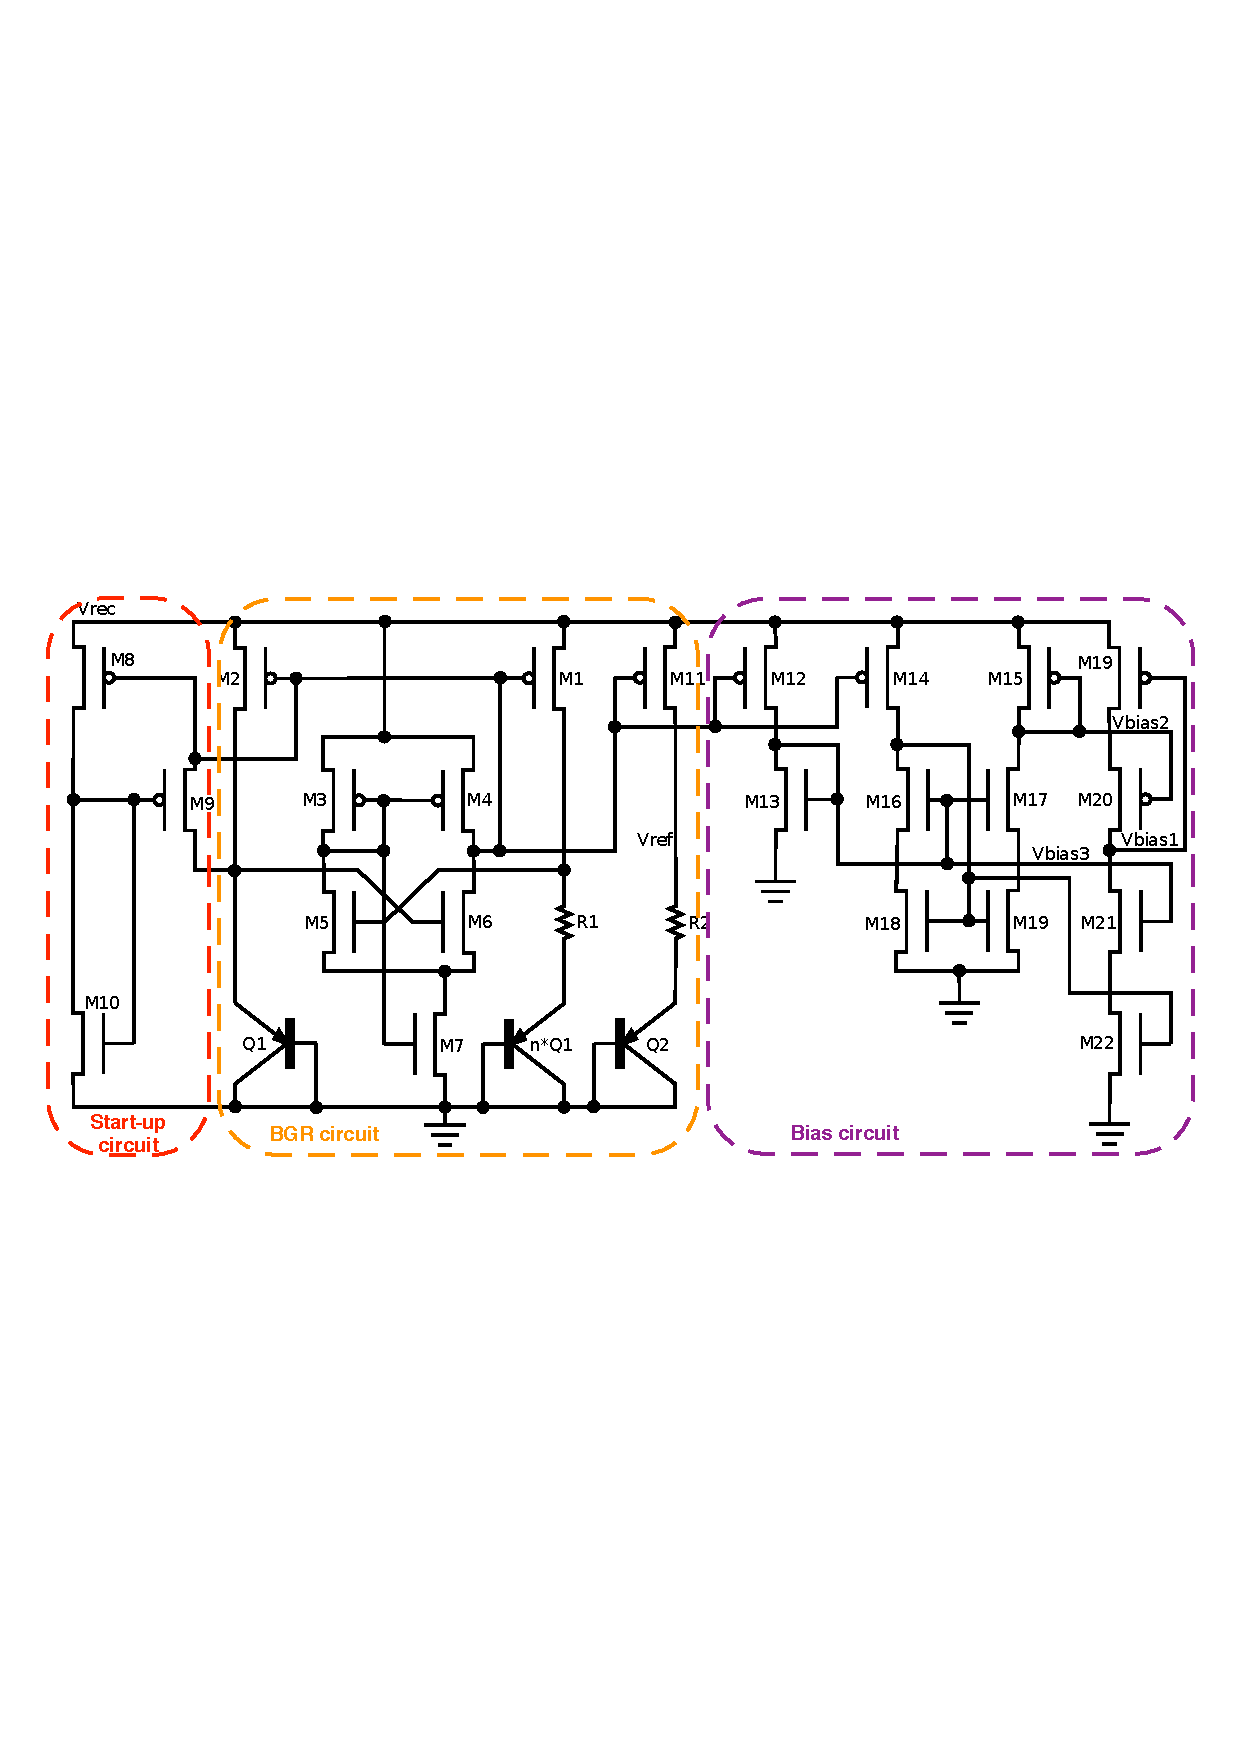
\includegraphics[width=\textwidth]{img/sch_bgr_label.pdf} 
   \caption{BGR and bias generation circuit}
   \label{bgr_sch}
\end{figure}

PTAT current is first generated using thermal voltage referenced current source using PNP transistor as diodes, resistor and a op-amp controlled current mirror \cite[pp. 391-392]{razavi_2001}. The current is $I = V_T ln(n)/R_1$, where $V_T = kT/q $ is thermal voltage with positive TC and $n$ is number of parallel PNP transistors. This current is passed through a resistor, $R_2$ to create a PTAT voltage which is in series with a diode realised with a parasitic PNP transistor. The value of $R_2$ is so chosen such that the positive TC of PTAT voltage across it is equal to negative TC of $V_{BE}$. The temperature independent reference voltage is then given as $V_{ref}  = V_{BE} + \alpha V_T ln(n)$, where $ \alpha = R_2/R_1$ is equal to $  \Delta V_{BE}/\Delta T$. Similarly the folded cascode  \gls{ota} working as an error amplifier in LDO requires additional bias voltages which are produced as shown. Wide swing current mirror topology is used here for bias voltage generation.\\

In case of the supply independent and self biased circuit, there may be start-up issue. If all the transistors carry zero current, they may indefinitely remain off even when the supply is turned on. Therefore start-up circuit is added in order to ensure that the devices are turn on as supply voltage is provided. Once the circuit is fully operational, the start-up circuit is off and does not effect the normal operation of BGR circuit. \\

Figure  \ref{bgr_temp}, \ref{bgr_dc} and \ref{bgr_tran} illustrates temperature, DC and transient simulation of the BGR circuit respectively for slow(ss), fast(ff) and typical(tt) corners. The plots shows that $V_{ref}$ is fairly independent with PVT variations. Similarly, $I_{bias}$ varaitons used for generating the bias voltages remains within condiderable range. Table \ref{bgr_spec} summarizes the performances of the BGR design. 

\begin{figure}[htbp] %figure placement: here, top, bottom, or page
   \centering
   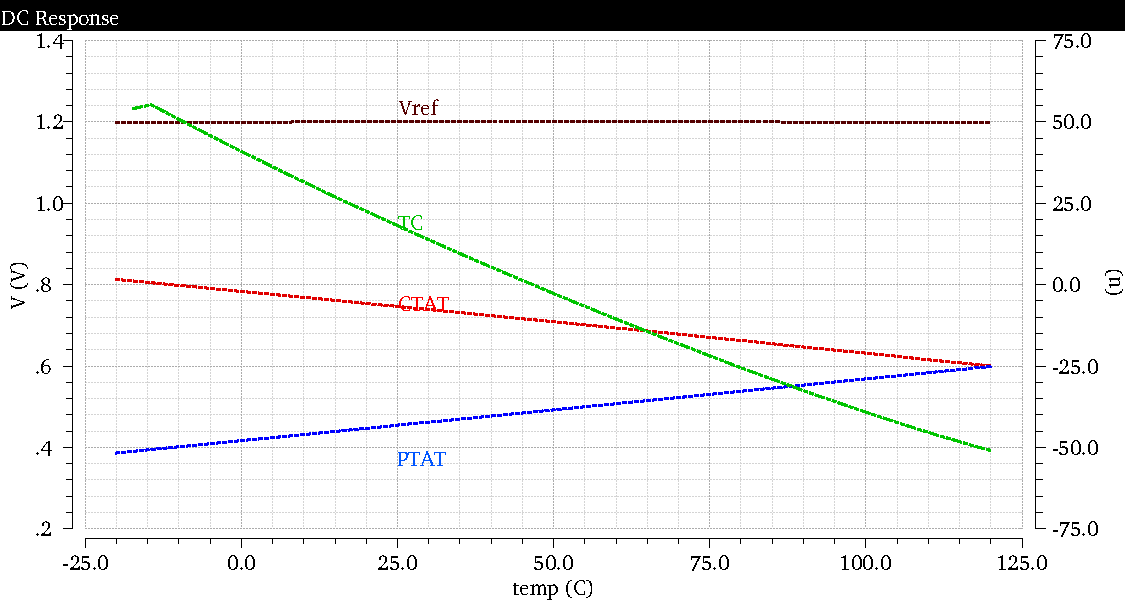
\includegraphics[width=0.9\textwidth]{img/bgr_temp.pdf} 
   \caption{BGR over temperature varitaion}
   \label{bgr_temp}
\end{figure}

\begin{figure}[htbp] %figure placement: here, top, bottom, or page
   \centering
   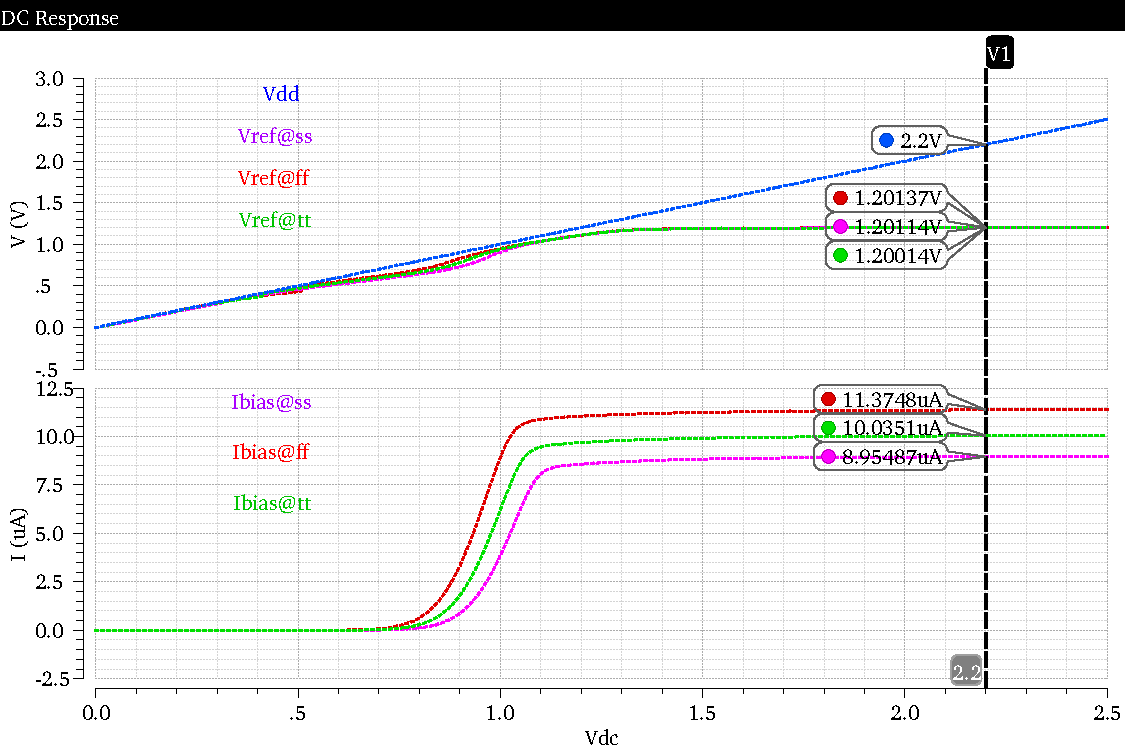
\includegraphics[width=0.9\textwidth]{img/bgr_dc.pdf} 
   \caption{BGR DC performance}
   \label{bgr_dc}
\end{figure}

\begin{figure}[htbp] %figure placement: here, top, bottom, or page
   \centering
   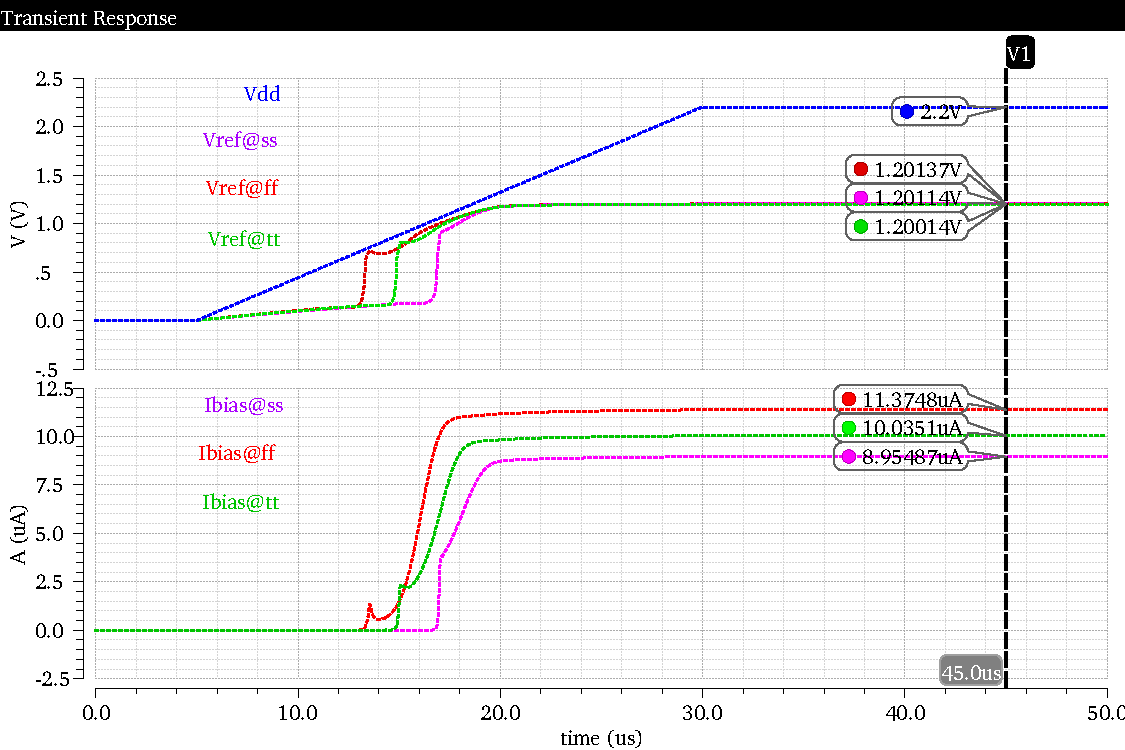
\includegraphics[width=0.9\textwidth]{img/bgr_tran.pdf} 
   \caption{BGR transient performance}
   \label{bgr_tran}
\end{figure}

\begin{table}[htbp]
\caption{BGR parameter and performance}
\begin{center}
\begin{tabular}{c|c}
\hline \hline
\multirow{3}{*}{V\textsubscript{ref}} & 1.201.1 \si{\volt} @slow corner \\ \cline{2-2}
& 1.201.4 \si{\volt} @fast corner \\ \cline{2-2} %\hline
& 1.200.1 \si{\volt} @typical corner \\ \hline
TC @27\textdegree C & 16.4 \si{\micro\volt}/\textdegree C \\ \hline
\multirow{3}{*}{I\textsubscript{bias}} & 8.95 \si{\micro\ampere} @slow corner \\ \cline{2-2}
& 11.37 \si{\micro\ampere} @fast corner \\ \cline{2-2}
& 10.04 \si{\micro\ampere} @typical corner \\ 
\hline \hline
\end{tabular}
\end{center}
\label{bgr_spec}
\end{table}%


\clearpage
\newpage
% *********************************************************************** ANTENNA DESIGN  ***********************************************************************

\section{Antenna Design}

All the components discussed above are part of any power management system which takes DC input from power line 
and creates regulated output as required. However, the objective here is to replace direct power line connection with 
wireless link. Since the intention is to just create a wireless power transfer link, the option which is easier to implement, 
convinent to operate and gives higher transfer efficiency is the primary choice here. And the literatures in wireless power 
transfer studies show inductive couling meets all these requirement. \\

Inductive coupling boils down to principle of electromagnetic induction. When alternating electirc current is passed through 
a coil, say primary, it generates alternating magnetic field. If another coil, say secondary, is placed in this changing 
magnetic field, alternating voltage/current is induced in the coil. In other word, power from primary coil is transferred 
wirelessly to secondary coil through magneic field and this is popularly known as inductive power transfer link. And this 
induced ac voltage is rectified and then used to power up the load. \\

The energy transfer efficiency between the coils depends on how much of the magnetic field generated by the primary is captured 
by the secondary coil. And the capture of magnetic field by the secondary coil in turn depends on shape and size of two coils, 
their separation and alignment. All these factors influencing the transfer efficiency collectively gives a quantity called 
coupling factor, $k$. A pefect inductive link has a coupling factor 1, which means all the magnetic flux genetated by primary 
is captured by secondary. However normally achieved coupling factor in practical inductive link is 0.3 and at best 0.5. So 
for better transfer of efficiency, some improvisation is done to the inductive link, so that efficiency is less affected by 
coil separation and alignment. This is done by tuning both the primary and secondary coil to same frequency i.e. creating 
resonance at some frequency so that coil coulpling is the strongest at that frequency. This method of creating better wireless 
energay transfer link is popuolarly known as magnetic resonance coupling.\\ 

In this project, first an antenna coil is designed and characterised. Then inductive link created using that antenna is studied 
and finally magnetic resonance technique is implemented to increase transfer efficiency at the operating frequency. The antenna 
dimensions are provided by Nordic Semiconductor which is one of their design already used in some application. Since having 
similar shape and size of antennas is important in gaining more transfer efficiency, the same antenna type is used as both 
primary and secondary coils. \\

\subsection{Inductor model}

Figure \ref{fig:ant_non_ideal} is a lumped model of a planar antenna/coil/inductor made on a PCB. $Rp$, series DC resistance of wire and $Cp$, 
inter-winding self capacitance. These parasitics determine quality factor and self resonance frequency, \acrshort{srf} of 
the antenna. The quality factor is given as $Q = \omega L/Rp$ and SRF as $SRF = 1/(\sqrt{LCp})$, for this simple model. \\


\begin{figure}[!htbp] %figure placement: here, top, bottom, or page
   \centering
   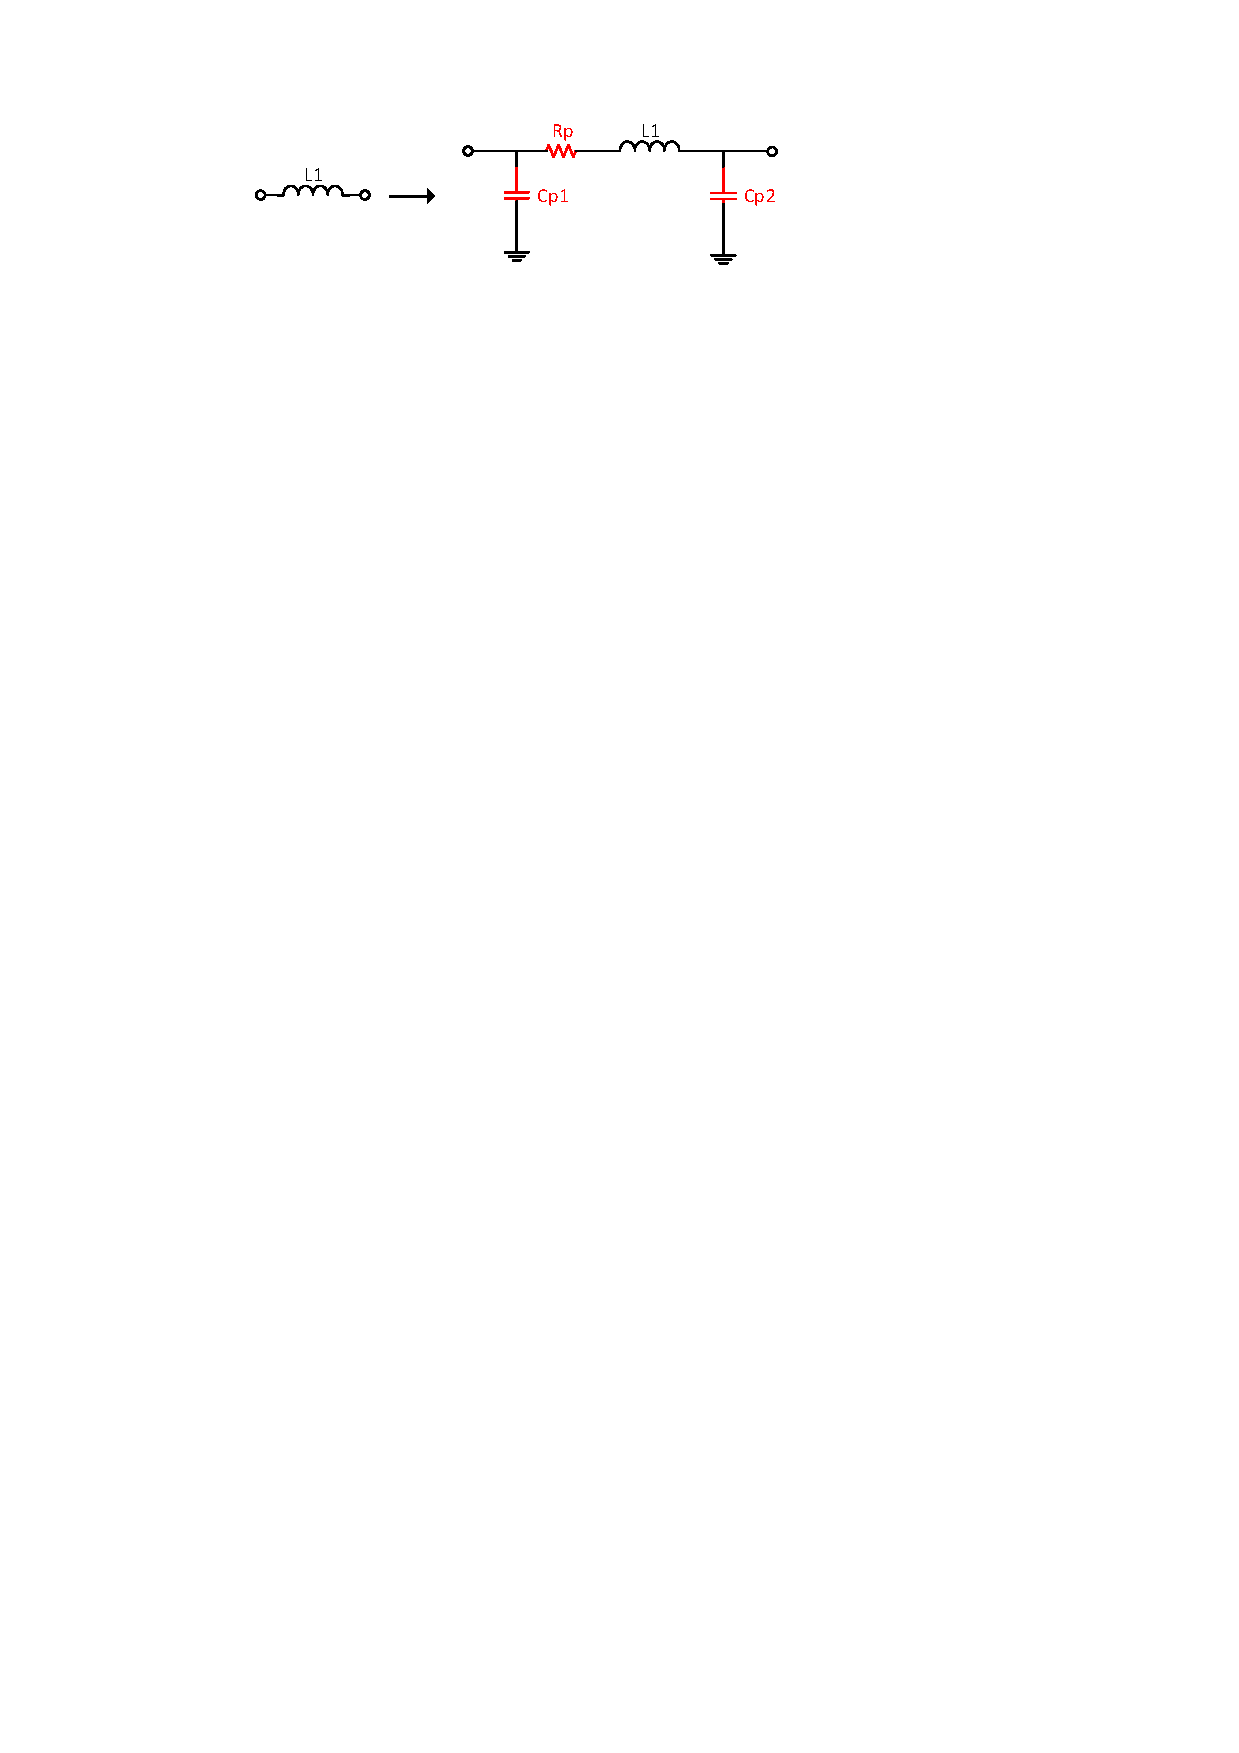
\includegraphics[width=0.9\textwidth]{img/ant_non_ideal.pdf} 
   \caption{Real antenna model}
   \label{fig:ant_non_ideal}
\end{figure}

For purpose of this work, with provided dimensions of the antenna, it is first modelled in HFSS as shown in 
figure \ref{fig:ant_single_model} and its equivalent lumped circuit in figure \ref{fig:ant_single_schematic}. It is important to 
note here that L1 in \ref{fig:ant_single_schematic} is in fact \ref{fig:ant_non_ideal}. However, in the discussion ahead, these 
parasitics are not explicitly mentioned because the parameter extraction will include these factors too. To realise a real antenna, physical parameters of materials used for making 
printed antenna on a PCB are also given for the model.  After completing model, frequency sweep is done for extracting S parameter of the 
antenna which was eventually used to estimate  self inductance of the modelled coil. The performance estimation of 
single antenna here and couple system later is based on formulas in \cite{ant_SZ_formula}. In order to check and compare the estimated inductance value from 
the model, Modified Wheeler Formula, a mathematical approximation model described in \cite{ant_inductance_calculation} is used. The 
qualities of antenna obtained from extracted S-parameter are listed in table \ref{tab:ant_inductance_compare}. The table shows that 
modelled inductance value is less than mathematically approximated value. This difference can be explained with two things. 
Firstly, mathematical calculation assumed that the antenna is spiral and rectangular with sharp edge but the model has 
rounded edge. Secondly, during modelling besides dimensions of the coils, physical parameters of coil materials are also used 
but these are not considered for mathematical calculation.\\

\begin{figure} [!htbp]
  \centering 
  \subfloat[HFSS antenna model]  {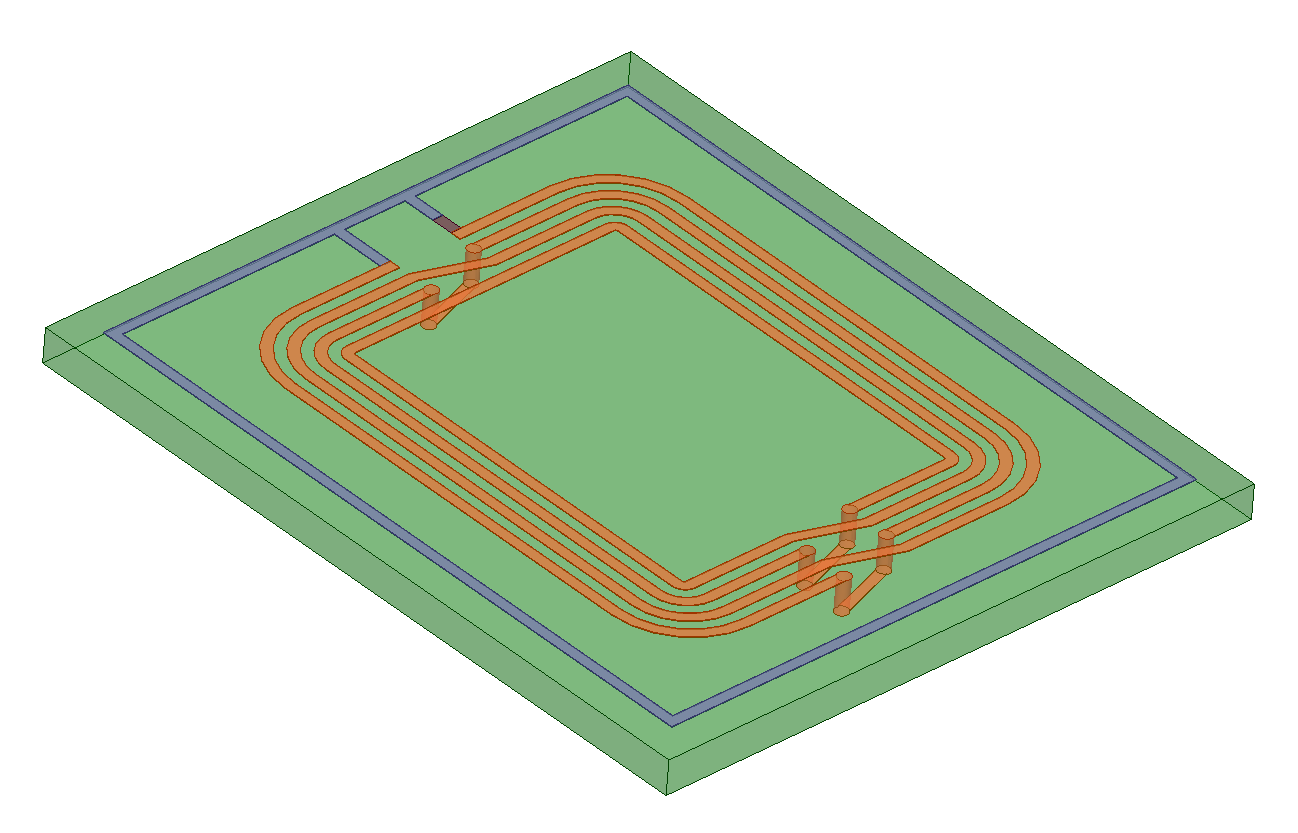
\includegraphics[width=.49\textwidth]{img/ant_single.png} \label{fig:ant_single_model}}
\hfill
 \subfloat[Equivalent schematic]  {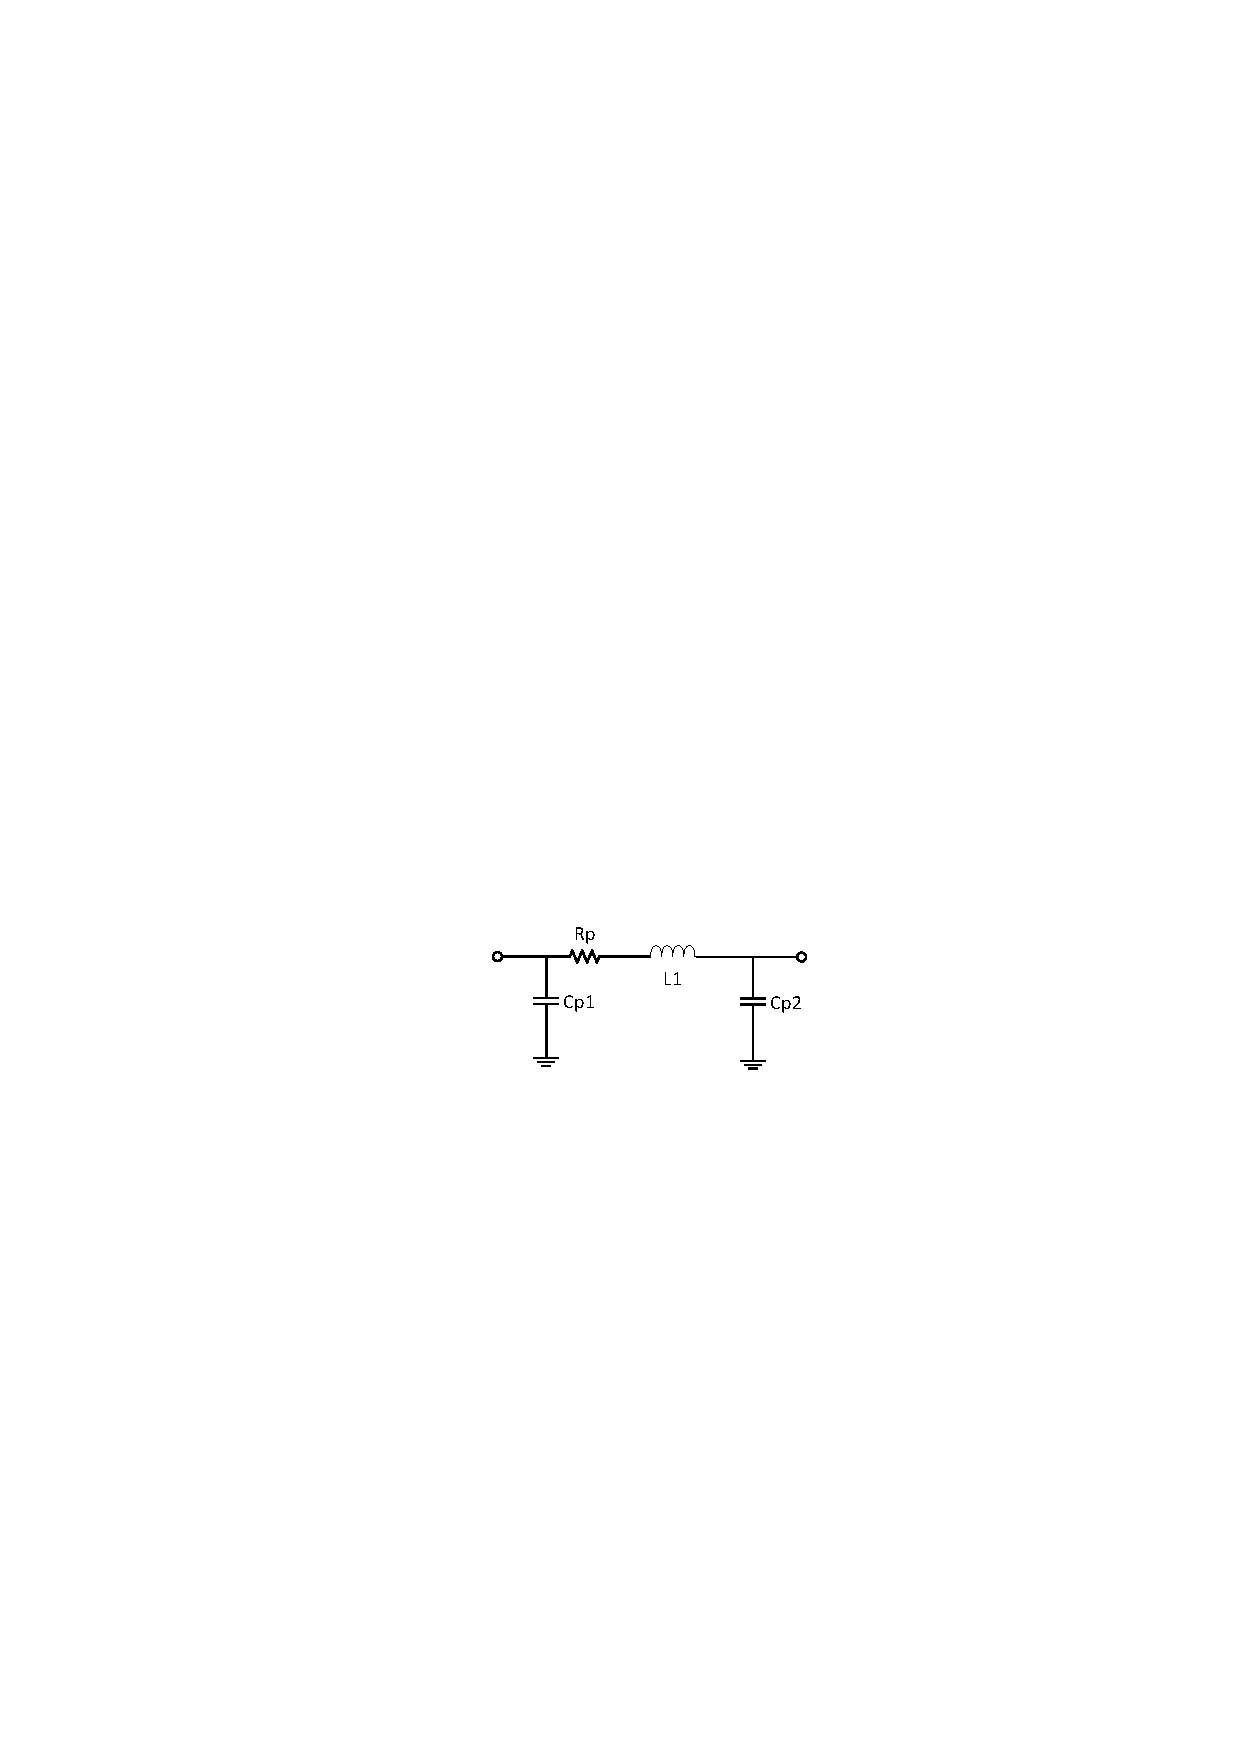
\includegraphics[width=.49\textwidth]{img/ant_single.pdf}\label{fig:ant_single_schematic}}
 \caption{Antenna model} 
\label{fig:ant_single} 
\end{figure}


\begin{table}[!htbp]
\caption{Characterisation of antenna} 
\begin{center}
\begin{tabular}{c|c|c}
\hline \hline
			& HFSS model 			& Modified Wheeler \cite{ant_inductance_calculation}  \\ \hline \hline
Self Inductance	  	& 448 \si{\nano\henry} 		& 644 \si{\nano\henry} \\ \hline
SRF		  	& 125 MHz			& 			\\ \hline
Quality factor		& 				&			\\ \hline
Parasitic Resistance	&				&			\\ \hline
Parasitic Capacitancce  &				&			\\
	  
\hline \hline
\end{tabular}
\end{center}
\label{tab:ant_inductance_compare}
\end{table}%

\subsection{Inducitve link: coupled coils}

In the next step, an inductive link is realised by using two antennas: one as primary and other as secondary, aligned one over 
other and separated by air gap as shown in figure  \ref{fig:ant_couple_model}, equivalently shown as lumped schematic in 
figure  \ref{fig:ant_couple_schematic}. Coupling system of these antennas is simulated for 
varying distance of magnetic field interaction to observe the difference in performance. The same procedure as 
used for single coil above, is used to extract self inductance of each coil, $L1$ and $L2$, mutual inductance 
of two coils, $L12$, coupling coefficient between the coils, $k$ and quality factor, $Q$. The extracted values for coil separation of 
1mm, 5mm and 10mm are listed in table \ref{tab:ant_couple_parameter} calculated at operating frequency of 13.56 MHz. \\


\begin{figure} [htbp]
  \centering 
  \subfloat[HFSS coupling model]  {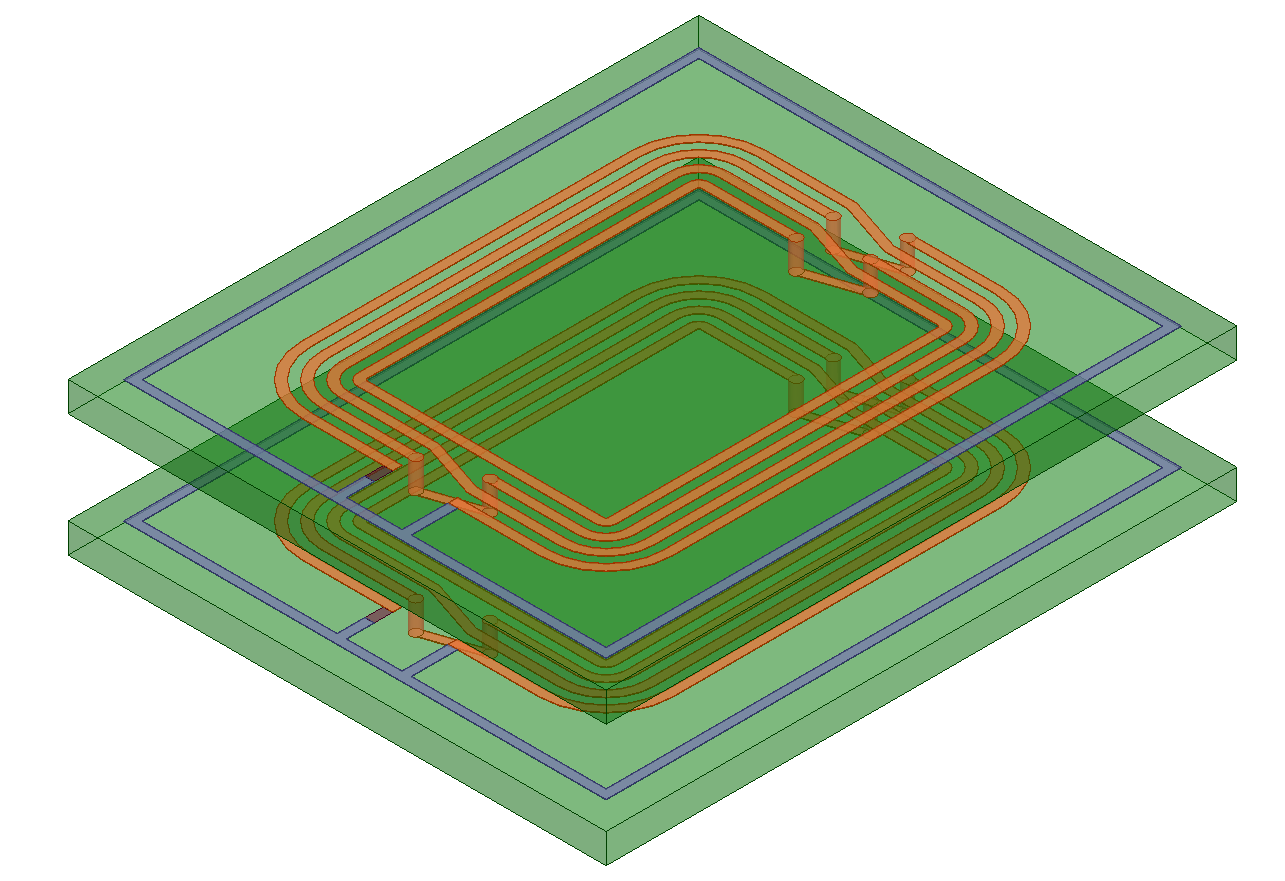
\includegraphics[width=.49\textwidth]{img/ant_couple.png} \label{fig:ant_couple_model}}
\hfill
 \subfloat[Equivalent schematic]  {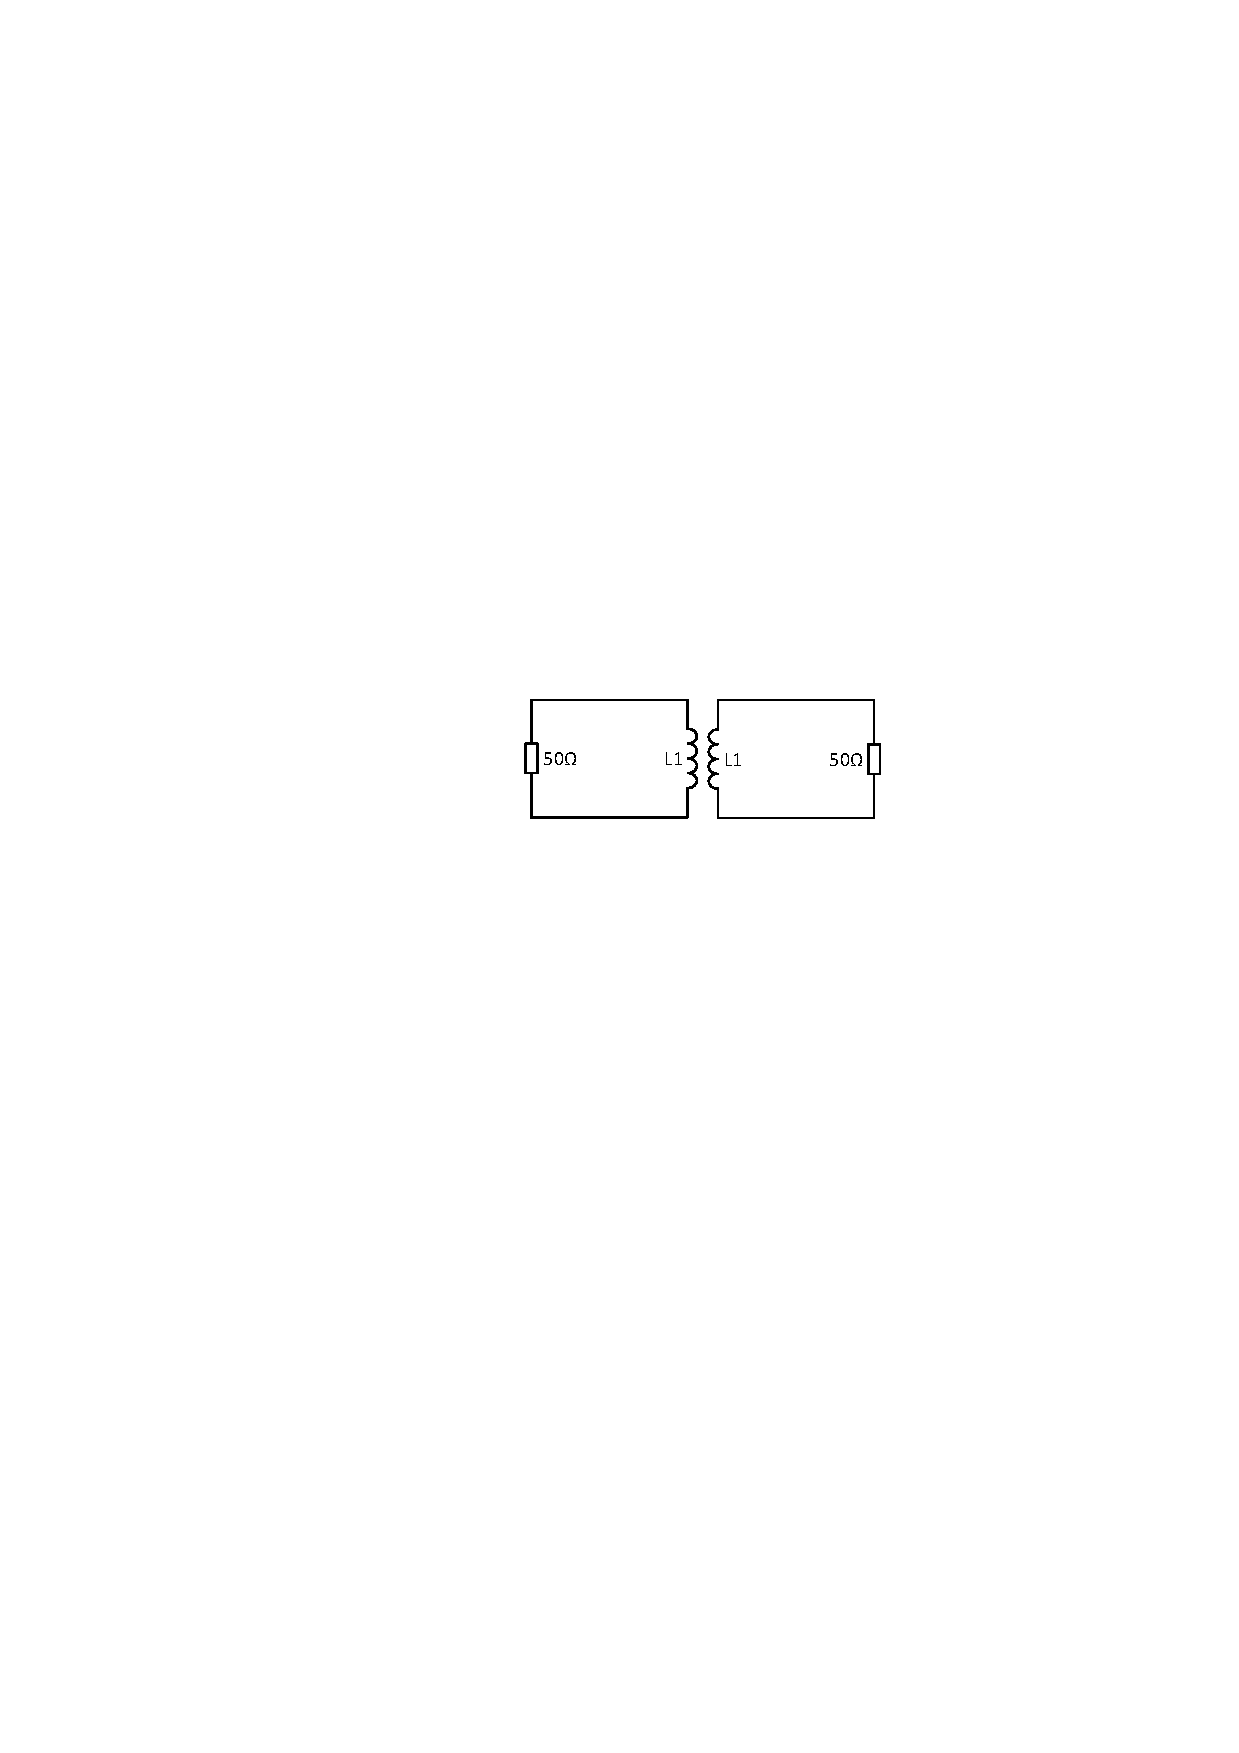
\includegraphics[width=.49\textwidth]{img/ant_couple.pdf}\label{fig:ant_couple_schematic}}
 \caption{Antenna coupling model} 
\label{fig:ant_couple} 
\end{figure}

\begin{table}[H]
\caption{Coupling parameters for varying coils distance} 
\begin{center}
\begin{tabular}{c|c|c|c|c}
\hline \hline
Parameter 	& 1 mm	& 5 mm 	& 10 mm	 & \si{\milli\meter}\\ \hline
L1		& -	& -	& -	 & \si{\nano\henry} \\ \hline
L2		& -	& -	& -	 & \si{\nano\henry} \\ \hline
L12		& -	& -	& -	 & \si{\nano\henry} \\ \hline
k		& -	& -	& -	 & -		    \\ \hline
Q		& -	& -	& -	 & -		    \\	\hline
SRF		&	&	&	 &		\\
\hline \hline
\end{tabular}
\end{center}
\label{tab:ant_couple_parameter}
\end{table}%

It is observed that $L1$ and $L2$ are same as in table \ref{tab:ant_inductance_compare} as it is the same coil used as primary 
and secondary. Similarly $L12$ and $k$, related as $L12 = k\sqrt(L1L2)$, are both decreasing with distance as expected. With 
increase in separation, less and less magnetic flux generated by primary coil is linked with the secondary, creating a loosley
coupled inductive link. \\

The power transfer efficiency of the physical link created by coupled coils is very important. [CITE] states 
that efficiency depends k of coupling system and Q of coil and hence high k and high Q is always desirable and obviously 
coil optimisation is the most important part of coupling system design. \cite{ant_optimal_resonance} and \cite{ant_PSC_geometry} 
discusses some techniques to optimise transfer efficiency of inductive link: \cite{ant_optimal_resonance} about matching the 
load for better resonance whereas \cite{ant_PSC_geometry} about designing optimal coil geometry for higher Q. The former one 
compares the efficiency of general inductive coupling and conventional resonant coupling and their limitation in achieving 
higher efficiency. This eventually proposes optimal resonant load transformation which has better immunity to poor coupling 
and load variation. Likewise, the later one describes step by step iterative process of designing an antenna with optimal geometry for the given 
design constraints. \\

\subsection{Magnetic Resonance Coupling}

In this project, conventional magnetic resonance coupling as in is implemented to tune both primary and secondary 
to the power career frequency. The purpose here is to match the impedance of primary antenna to source impedance and secondary antenna of 
coupling system to load impedance in order to maximize the power tramsmission from the source to  the load.  \\


For the purpose of making a resonant inductive link, the S parameter of coupled antenna system in HFSS 
is exported to ADS in order to design matching networks using capacitors only. Impedance of  primary antenna is 
matched to 50 \si{\ohm} source resistance and impedance of secondary is matched to load impedance (50 \si{\ohm} load or input 
impedance chip(?)) as shown in \ref{fig:ant_couple_resonant}. $Cp1$, series capacitor and $Cp2$, shunt capacitor together 
with $L1$ created parallel resonant circuit at 13.56 MHz on the primary side and $Cs1$, shunt capacitor together with $L2$ 
creates the secondary resonant circuit at same operating frequency. Thus a pair of LC tank circuit is made tuned at same 
frequency. Such matching network is designed for all three coil separation distances as above, but resonant coupling system 
with 5 mm separation is taken as a typical example and presented here. \\

The reflection power loss, S11 and S22, at both primary and secondary terminal, power transfer gain, S21, from primary 
to secondary and Q-factors for both antennas before and after creating resonance are shown in figure \ref{fig:ant_S_loss}, 
this and this. \\


\begin{figure}[!htbp] %figure placement: here, top, bottom, or page
   \centering
   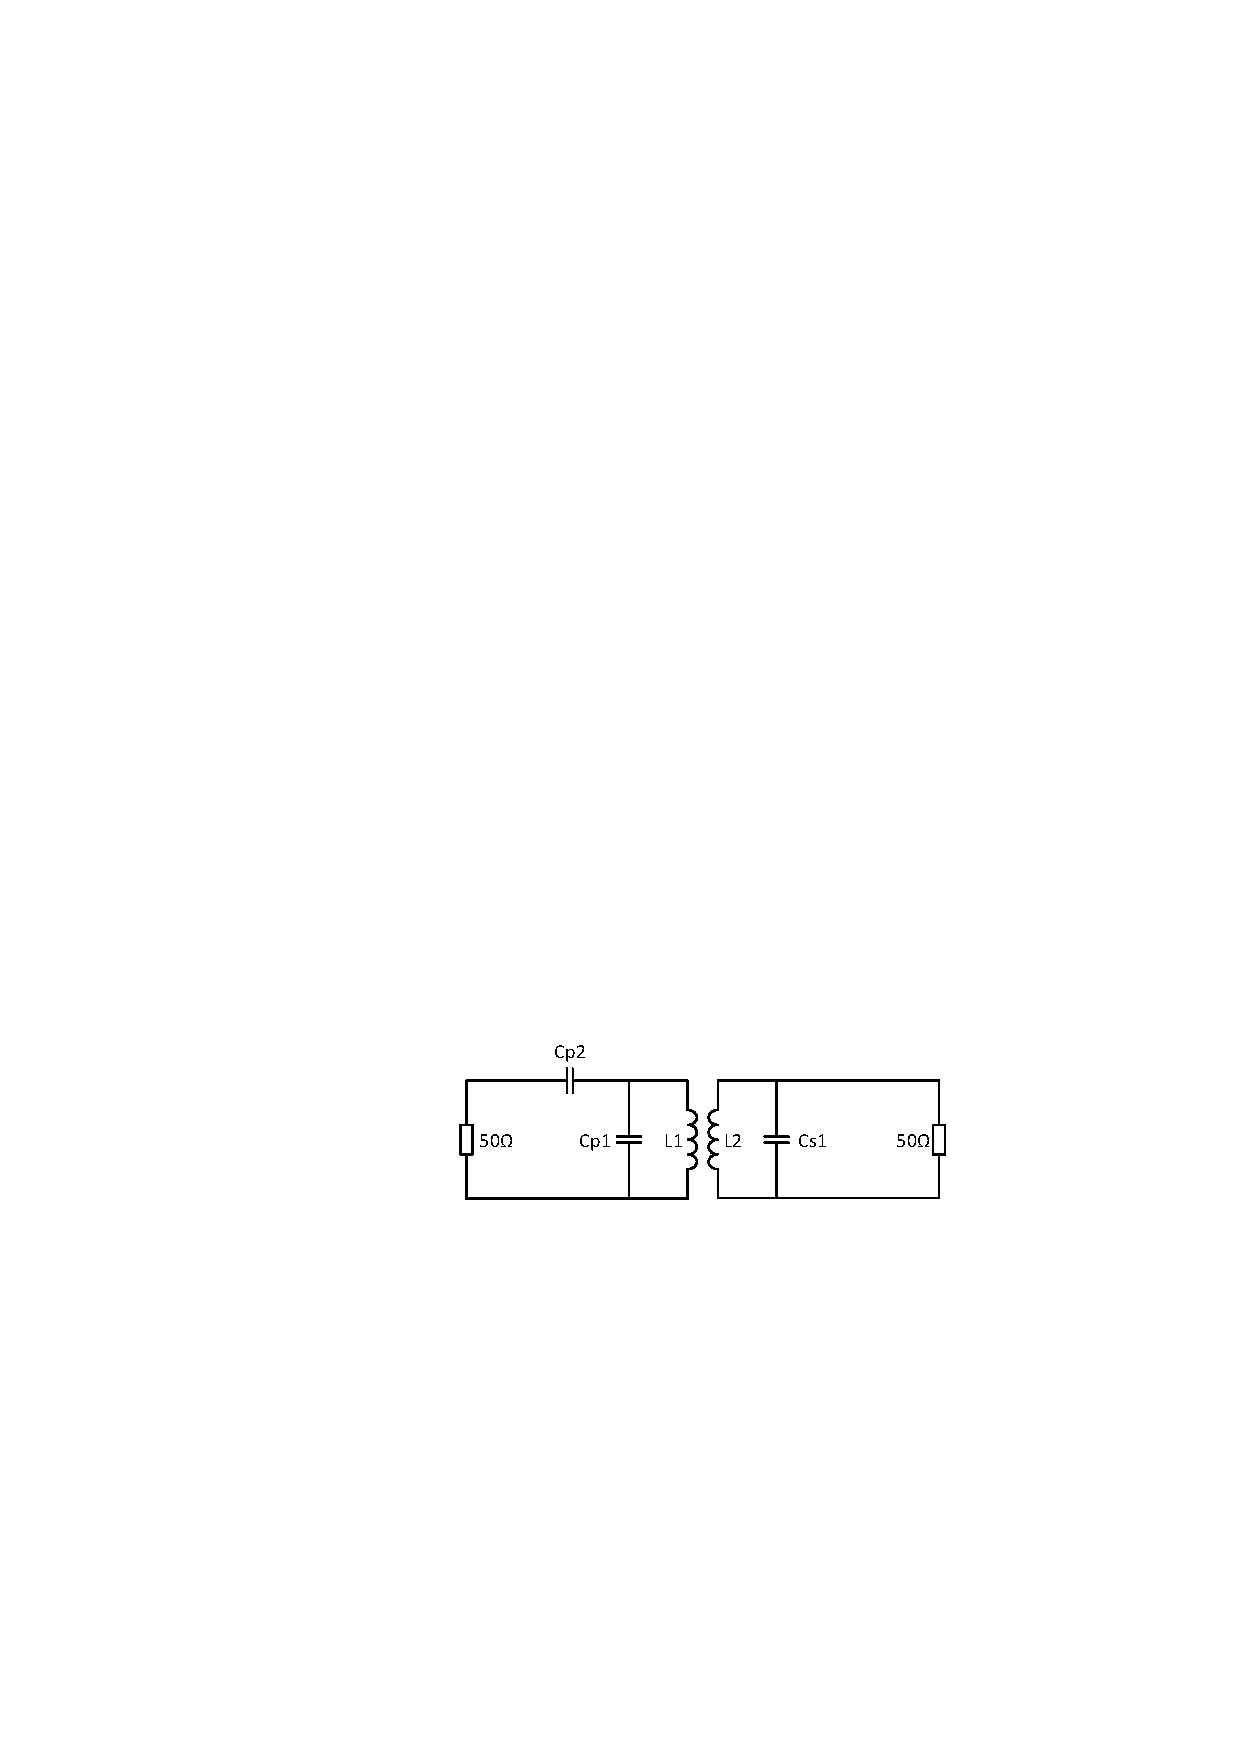
\includegraphics[width=0.8\textwidth]{img/ant_couple_resonant.pdf} 
   \caption{Resonant coupled inductive link}
   \label{fig:ant_couple_resonant}
\end{figure}

\begin{figure} [!htbp]
  \centering
  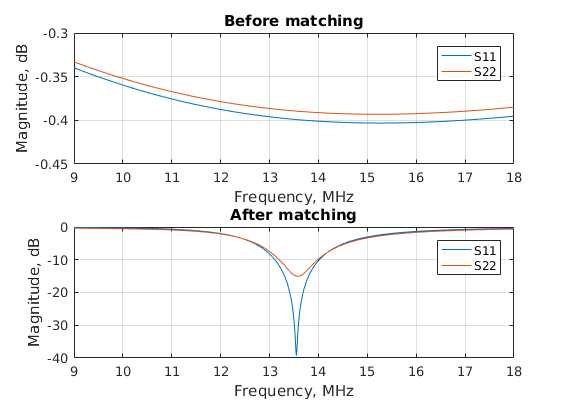
\includegraphics[width=0.9\textwidth]{img/ant_S_loss.png} 
 \caption{Power loss before and after matching} 
\label{fig:ant_S_loss} 
\end{figure}

The performance of magnetic resonant coupling link designed in this work is summarises in table \ref{tab:ant_spec} below.

\begin{table}[!htbp]
\caption{Performance of resonant inductive link} 
\begin{center}
\begin{tabular}{c|c}
\hline \hline
$Cp1$ $Cp2$ and $Cs1$	  	& 			\\ \hline
Resonant frequency		& 13.56 MHz		\\ \hline
Primary reflection loss		&			\\ \hline
Secondary reflection loss	& 			\\ \hline
Primary to secondary gaining	& 			\\ \hline
Q-factor			&			\\
\hline \hline
\end{tabular}
\end{center}
\label{tab:ant_spec}
\end{table}%

\clearpage
\newpage
% *********************************************************************** WPT PRU SYSTEM  ***********************************************************************


\section{Power Receiving Unit}
Wireless power transfer, \acrshort{wpt} system always constitutes two main units: power transmitting unit, 
\acrshort{ptu} and power receiving unit, \acrshort{pru}. Each unit comprises of resonator, power conditioner 
and control circuits as shown in figure [figure]. Both the resonators in PRU and PTU are tuned to operating 
frequency, which create a physical transfer link. Power conditioner circuit in PTU includes at least power 
amplifier and matching circuit, whereas in PRU, it includes matching curcuit, recitifier and regulator. 
Similarly both these units have control block which faciliates transfer procedure and communication between 
these units.  In this work design and analysis of PRU is the main objective. Since PRU cannot be realised 
without a transfer link, primary antenna creates a very simply PTU here.  \\

Figure [FIGURE] is the block diagram of PRU system in this design. Secondary coil is the receiver resonator and  
rectifer, LDO and reference and biasing is power conditioning block. The primary coil is 
driven by a power source and AC signal is generated at the secondary as discussed earlier in antenna design 
section. The rectifer then rectifies this AC singnal to DC. The DC output of the rectifer is then fed to LDO 
to produce regulated DC output required to drive a load. The reference and biasing circuit generates required 
reference and biasing DC voltages for the LDO. \\

The simulation of the PRU system is done is two steps. As this system can be functionally divided into two sub-system: 
coupling system and Power Management System (\acrshort{pms}), fisrtly PMS is simulated excluding the coupled antennas 
to characterise the performace of PMS. Secondly, the whole PRU system: PMS with coupled antenna is simulated to observe 
the wireless power transfer and then management of this transferred power. Though it has already been told earlier, 
one important thing must be mentioned here again before going further. Even though reference and biasing circuit has 
been integrated into the PMS system, it has been designed with an option to override it externally. This externally 
supplied reference and biasing will be primarily used for the PRU system simulation. The result with on-system baises 
and reference will be explicitly noted when used. \\

Figure [FIGURE] is testbench setup for PMS simualtion. PMS block in the picture includes rectifer, LDO and RB. The values external 
biases and references and off-chip components are listed in table [TABLE]. The requirement and choice of these components 
are described in their respecitve design section above.



\clearpage
\newpage
\nocite{*}
\printbibliography

\newpage
\listoffigures

\newpage
\listoftables

%\printindex
\newpage
\printnoidxglossaries

\end{document}